
% Module 3: Gauge Symmetry and Construction of the Standard Model

\documentclass[11pt,a4paper]{article}

\usepackage[a4paper,margin=1in]{geometry}
\usepackage[T1]{fontenc}
\usepackage[utf8]{inputenc}
\usepackage{newtxtext,newtxmath}
\usepackage{microtype}
\usepackage{xcolor}
\usepackage{graphicx}
\usepackage{tikz}

%\usetikzlibrary{arrows.meta,positioning,calc,fit,shapes.geometric,decorations.pathmorphing,backgrounds}

\usetikzlibrary{matrix,arrows.meta,positioning,calc,fit,shapes.geometric,decorations.pathmorphing,backgrounds}

\usepackage{amsmath,mathtools,bm}
\usepackage{enumitem}
\usepackage{booktabs,tabularx,array,longtable,multirow}
\usepackage{caption}
\usepackage{titlesec}
\usepackage{fancyhdr}
\usepackage{hyperref}
\usepackage[most]{tcolorbox}
\usepackage{float}
\usepackage{csquotes}
\usepackage{setspace}
\usepackage{array}

\hypersetup{colorlinks=true,linkcolor=blue!50!black,urlcolor=blue!50!black,citecolor=blue!50!black}

\definecolor{aghblue}{RGB}{95,105,175}
\definecolor{aghlight}{RGB}{236,238,255}
\definecolor{aghdark}{RGB}{35,35,35}
\definecolor{softgray}{RGB}{246,246,246}
\definecolor{accentgreen}{RGB}{68,110,90}
\definecolor{accentred}{RGB}{145,70,78}
\definecolor{accentorange}{RGB}{176,108,24}

\setstretch{1.08}
\setlength{\parindent}{0pt}
\setlength{\parskip}{0.65em}

\pagestyle{fancy}
\fancyhf{}
\fancyhead[L]{\small\itshape Module 3: Gauge Symmetry and Construction of the Standard Model}
\fancyhead[R]{\small The Standard Model} % - Technical Physics MSc}
\fancyfoot[C]{\thepage}
\renewcommand{\headrulewidth}{0.3pt}



\titleformat{\section}{\Large\bfseries\color{aghdark}}{\thesection}{0.75em}{}
\titleformat{\subsection}{\large\bfseries\color{aghdark}}{\thesubsection}{0.65em}{}
\titleformat{\subsubsection}{\normalsize\bfseries\color{aghdark}}{\thesubsubsection}{0.6em}{}



\newtcolorbox{guidelinebox}{enhanced,colback=white,colframe=aghblue!50,boxrule=0.8pt,
  sharp corners,left=8pt,right=8pt,top=8pt,bottom=8pt,
  overlay={\node[fill=aghlight,anchor=west,font=\bfseries] at ([xshift=8pt,yshift=-8pt]frame.north west){The Guideline};}}



\newtcolorbox{takehomebox}{enhanced,colback=softgray,colframe=accentgreen!65!black,boxrule=0.8pt,
  sharp corners,left=8pt,right=8pt,top=8pt,bottom=8pt,
  overlay={\node[fill=white,anchor=west,font=\bfseries\color{accentgreen!70!black}] at ([xshift=8pt,yshift=-8pt]frame.north west){Take-home message};}}



\newtcolorbox{guidedchecksbox}{enhanced,colback=white,colframe=accentorange!70!black,boxrule=0.8pt,
  sharp corners,left=8pt,right=8pt,top=10pt,bottom=8pt,
  overlay={\node[fill=white,anchor=west,font=\bfseries\color{accentorange!80!black}] at ([xshift=8pt,yshift=-8pt]frame.north west){Guided checks};}}



\newtcbtheorem[number within=section]{definition}{Definition}{enhanced,colback=white,colframe=aghblue!55,
  fonttitle=\bfseries,coltitle=black,colbacktitle=aghlight,boxrule=0.8pt,sharp corners,
  attach boxed title to top left={xshift=0.5em,yshift*=-2mm},boxed title style={sharp corners,colframe=aghblue!55,colback=aghlight}}{def}



\newtcbtheorem[number within=section]{remarkbox}{Remark}{enhanced,colback=softgray,colframe=black!35,
  fonttitle=\bfseries,coltitle=black,colbacktitle=black!5,boxrule=0.6pt,sharp corners,
  attach boxed title to top left={xshift=0.5em,yshift*=-2mm},boxed title style={sharp corners,colframe=black!35,colback=black!5}}{rem}



\newtcbtheorem[number within=section]{examplebox}{Example}{enhanced,colback=white,colframe=accentred!55,
  fonttitle=\bfseries,coltitle=black,colbacktitle=accentred!10,boxrule=0.8pt,sharp corners,
  attach boxed title to top left={xshift=0.5em,yshift*=-2mm},boxed title style={sharp corners,colframe=accentred!55,colback=accentred!10}}{ex}

\newcommand{\Lag}{\mathcal{L}}
\newcommand{\ii}{\mathrm{i}}
\newcommand{\ee}{\mathrm{e}}
\newcommand{\dd}{\mathrm{d}}
\newcommand{\p}{\partial}
\newcommand{\Tr}{\mathrm{Tr}}
\newcommand{\diag}{\mathrm{diag}}
\newcommand{\comm}[2]{\left[#1,#2\right]}
\newcommand{\acomm}[2]{\left\{#1,#2\right\}}
\newcommand{\half}{\tfrac12}
\newcommand{\gmu}{\gamma^\mu}
\newcommand{\gnu}{\gamma^\nu}
\newcommand{\gfive}{\gamma^5}
\newcommand{\PL}{P_{\mathrm{L}}}
\newcommand{\PR}{P_{\mathrm{R}}}
\newcommand{\SLashed}[1]{#1\!\!/}
\newcommand{\SU}{\mathrm{SU}}
\newcommand{\Ug}{\mathrm{U}}
\newcommand{\SMgauge}{\mathrm{SU}(3)_c \times \mathrm{SU}(2)_L \times \mathrm{U}(1)_Y}
\newcommand{\SUc}{\mathrm{SU}(3)_c}
\newcommand{\SUw}{\mathrm{SU}(2)_L}
\newcommand{\UY}{\mathrm{U}(1)_Y}
\newcommand{\Qop}{Q}
\newcommand{\Tthree}{T_3}
\newcommand{\Yop}{Y}
\newcommand{\psibar}{\overline{\psi}}
\newcommand{\vev}[1]{\left\langle #1 \right\rangle}
\newcommand{\abs}[1]{\left|#1\right|}
\newcommand{\norm}[1]{\left\lVert #1\right\rVert}
\newcommand{\mc}[1]{\mathcal{#1}}
\newcommand{\figplaceholder}[2]{\begin{center}\fbox{\parbox[c][0.18\textheight][c]{0.78\textwidth}{\centering\bfseries #1\\[0.5em]\normalfont #2}}\end{center}}



\begin{document}


\begin{titlepage}
\centering
\vspace*{1.2cm}
{\textbf{AGH University of Krakow}\par}
{\textbf{Faculty of Physics and Applied Computer Science}\par}
\vspace{1.4cm}

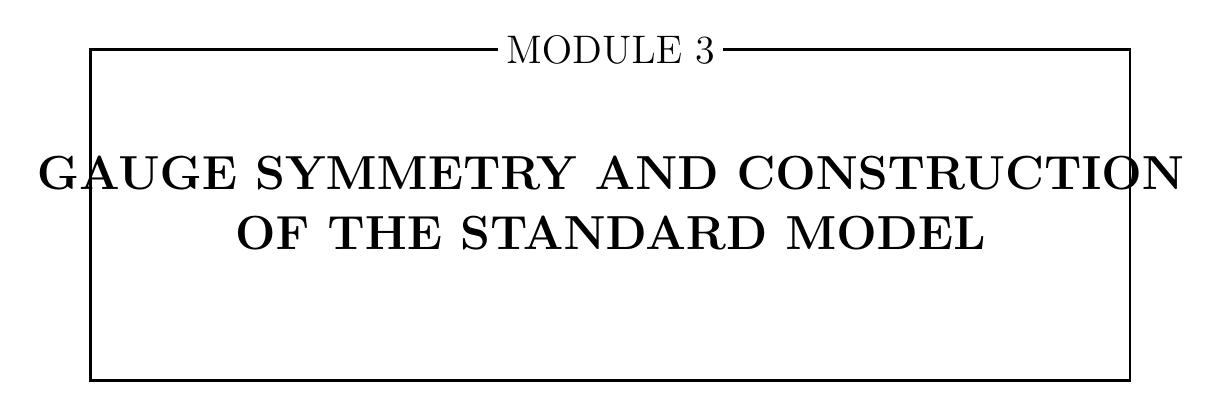
\begin{tikzpicture}
\draw[line width=0.9pt] (0,0) rectangle (13.2,4.2);
\node[fill=white,inner sep=3pt,font=\Large] at (6.6,4.2) {MODULE 3};
\node[font=\bfseries\fontsize{18}{22}\selectfont,align=center] at (6.6,2.25) {GAUGE SYMMETRY AND CONSTRUCTION\\OF THE STANDARD MODEL};
\end{tikzpicture}

\vspace{1.3cm}
{\Large Supporting Lecture Notes for \textit{The Standard Model}\par}
\vspace{0.35cm}
%{\large Technical Physics - Second-cycle Programme\par}
\vspace{1.2cm}




\begin{guidelinebox}
\vspace{0.25cm}
\itshape
The aim of this expanded module note is to make visible the constructive logic of gauge theory. Starting from global internal symmetry, we promote symmetry parameters to functions of spacetime, discover why the ordinary derivative fails, and are led naturally to the covariant derivative and the gauge field. Quantum electrodynamics then appears as the prototype Abelian gauge theory. The same logic is subsequently generalized to non-Abelian Yang--Mills theory and finally to the Standard Model gauge structure {\color{red}\(\SMgauge\)}. Throughout the note, the emphasis is on seeing the Standard Model as a highly constrained framework whose interaction structure is determined by gauge invariance, field content, and representation theory.
\end{guidelinebox}



\vfill
{\normalsize Prepared for the Standard Model course\par}
{\textbf{Hamzeh Khanpour}\par}
{\normalsize \texttt{hamzeh.khanpour@fis.agh.edu.pl}\par}
{\texttt{https://view.fis.agh.edu.pl/staff/hamzeh.khanpour/}\par}
{\normalsize \today\par} % {\normalsize April 7, 2026\par}

\end{titlepage}



\tableofcontents


\newpage



\section*{Preface}
\addcontentsline{toc}{section}{Preface}

These expanded supporting notes are written for \textit{Module 3: Gauge Symmetry and Construction of the Standard Model}. The pedagogical goal is not only to present the main formulas of gauge theory, but to guide the reader through the logic that connects them. The whole note is organized around a single constructive chain:
\[
\text{global symmetry}
\longrightarrow
\text{local symmetry}
\longrightarrow
\text{covariant derivative}
\longrightarrow
\text{gauge field}
\longrightarrow
\text{field strength}
\longrightarrow
\text{gauge-invariant Lagrangian}.
\]
In the first half of the note, this chain is developed using the simplest possible example, the local \(U(1)\) symmetry of a Dirac field. In the second half, the same logic is generalized to Yang--Mills theory and then applied to the Standard Model gauge group and its matter content.

The note is designed to be self-contained at the level of a serious MSc student. It assumes familiarity with the Dirac equation, relativistic notation, and the basic language of quantum mechanics and field theory, but it does not assume that the reader has already internalized the gauge-theory viewpoint. For this reason, several short worked examples and guided checks are included. They are not intended as formal exercises in the textbook sense; rather, they are meant to help the reader test whether each structural step has really been understood.

It is equally important to keep the boundaries of the module explicit. These notes develop the gauge principle, QED as the prototype gauge theory, the Yang--Mills generalization, and the pre-electroweak-symmetry-breaking structure of the Standard Model. They do \emph{not} attempt to replace later modules on QCD phenomenology, asymptotic freedom, confinement, or electroweak symmetry breaking. Those topics are previewed only insofar as they help clarify why Module~3 matters.



\section*{Conventions and notation}
\addcontentsline{toc}{section}{Conventions and notation}

\begin{itemize}[leftmargin=1.7em]
\item Metric signature: \(\eta_{\mu\nu}=\diag(1,-1,-1,-1)\).
\item Clifford algebra: \(\acomm{\gamma^\mu}{\gamma^\nu}=2\eta^{\mu\nu}\).
\item Chirality projectors: \(\PL=(1-\gfive)/2\), \(\PR=(1+\gfive)/2\).
\item Abelian covariant derivative: \(D_\mu=\p_\mu-\ii q A_\mu\).
\item Non-Abelian covariant derivative: \(D_\mu=\p_\mu-\ii g A_\mu\), with \(A_\mu=A_\mu^a T^a\).
\item Hypercharge convention: \(\Qop=\Tthree+\Yop\).
\item Generator normalization in the fundamental representation: \(\Tr(T^aT^b)=\half\delta^{ab}\).
\end{itemize}



\newpage




\section{Introduction and module roadmap}

\subsection{Why gauge symmetry is a construction principle}

The Standard Model is often introduced through a chart of particles: quarks, leptons, gauge bosons, and the Higgs boson. Such a chart is useful as a summary, but it can also be misleading pedagogically. A chart tells us \emph{what} appears in the theory, but it does not explain \emph{why} the theory takes the form it does. It does not explain why quarks come in color triplets, why weak interactions distinguish left and right, why gauge bosons self-interact in some sectors but not in others, or why electric charge is related to weak isospin and hypercharge by a precise algebraic rule.

The deeper viewpoint is that the Standard Model is a relativistic \emph{chiral gauge theory}. Its structure is not built by writing down all possible interactions and then discarding those that fail experimentally. Instead, one begins with a small number of organizing principles: relativistic covariance, locality, quantum fields carrying internal symmetry labels, and the requirement that certain symmetries be local rather than merely global. These principles are so restrictive that they force the theory into a highly nontrivial form.

This is why gauge symmetry deserves to be called a construction principle. A global internal symmetry may already imply a conserved quantity, but it does not yet force the introduction of a new interaction field. A local symmetry does. Once the transformation parameter depends on spacetime, the ordinary derivative fails to transform covariantly, and the theory can no longer be written consistently in its original form. To repair the failure, one is compelled to introduce a gauge field and a covariant derivative. The interaction is therefore not an optional embellishment; it is the price of local covariance.



\subsection{From Module 2 to Module 3}

Module~2 developed the language of relativistic fermions. There the emphasis was on how spin-\(\half\) fields are described consistently in relativistic quantum theory, how the Dirac equation is constructed, and how chirality emerges naturally in the relativistic setting. Those ideas are indispensable preparation for the present module, because the gauge principle does not act on abstract objects in isolation. It acts on fields that already possess a well-defined Lorentz and spinor structure.

The conceptual question of Module~3 can therefore be stated very simply: given the relativistic matter fields introduced in Module~2, how can one couple them to interactions in a way that respects locality and symmetry? The answer is not to invent a coupling term directly. Instead, one searches for a more fundamental criterion that determines what kind of coupling is allowed. That criterion is local gauge invariance.




\subsection{What this module will and will not do}

This module develops in full the chain
\[
\begin{aligned}
\text{global symmetry}
&\longrightarrow \text{local symmetry}
\longrightarrow \text{failure of } \partial_\mu \\
&\longrightarrow \text{covariant derivative}
\longrightarrow \text{gauge field}
\longrightarrow \text{QED} \\
&\longrightarrow \text{Yang--Mills theory}
\longrightarrow \text{Standard Model gauge structure}.
\end{aligned}
\]
In particular, it gives detailed attention to the transition from global to local symmetry, to the construction of the Abelian gauge theory of electrodynamics, to the minimal Lie-algebra toolkit required for non-Abelian symmetry, and to the pre-electroweak-symmetry-breaking structure of the Standard Model.

At the same time, the module intentionally stops short of several important later topics. It does not develop the phenomenology of QCD in detail, nor does it attempt a full treatment of spontaneous symmetry breaking, the Higgs mechanism, Yukawa couplings, or the physical \(W^\pm\), \(Z\), and photon mass eigenstates. Those topics belong mainly to later modules. Here the focus is on the construction of the gauge theory itself.




\subsection{Roadmap of the note}

The note proceeds in four broad movements. First, we review global internal symmetry using the free Dirac field as the simplest concrete example. This yields a conserved Noether current but no interaction field. Second, we promote the symmetry parameter to a function of spacetime and show explicitly where the ordinary derivative fails. This is the point at which the covariant derivative and the gauge field become necessary.

Third, we develop the resulting Abelian gauge theory in some detail, treating QED as the prototype theory in which the gauge principle can be seen in a complete form. Fourth, we generalize the construction to non-Abelian gauge symmetry and then apply the Yang--Mills framework to the Standard Model gauge group, matter multiplets, charge assignments, and gauge-sector Lagrangian before electroweak symmetry breaking.

\begin{figure}[H]
\centering
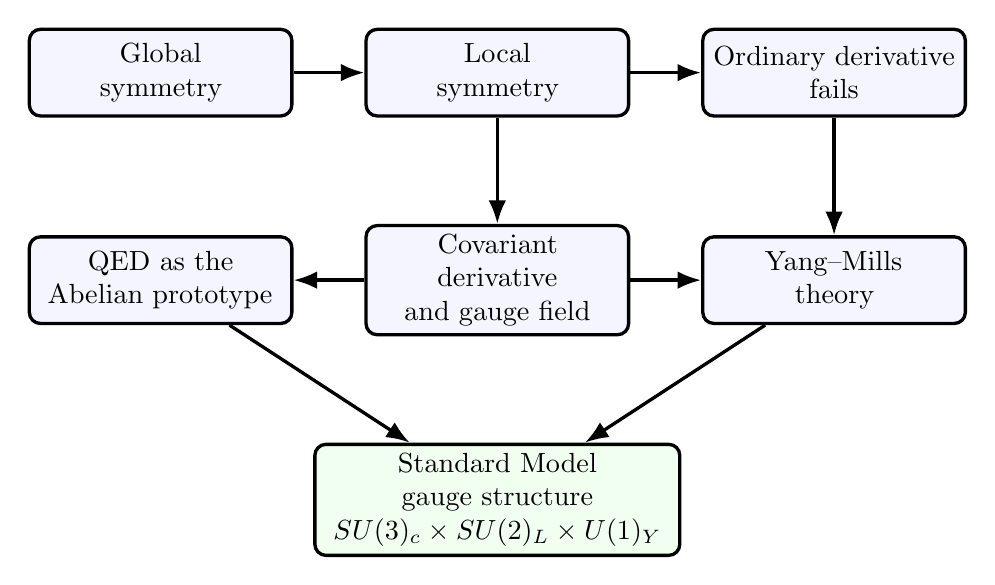
\begin{tikzpicture}[
	node distance=1.35cm and 0.9cm,
	block/.style={rounded corners, draw=black, very thick, align=center, minimum height=1.1cm, text width=3.1cm, fill=blue!4},
	arr/.style={-{Latex[length=3mm]}, very thick}
	]
	\node[block] (g) {Global\\symmetry};
	\node[block, right=of g] (l) {Local\\symmetry};
	\node[block, right=of l] (d) {Ordinary derivative\\fails};
	\node[block, below=of l] (c) {Covariant derivative\\and gauge field};
	\node[block, left=of c] (qed) {QED as the\\Abelian prototype};
	\node[block, right=of c] (ym) {Yang--Mills\\theory};
	\node[block, below=of c, text width=4.4cm, fill=green!6] (sm) {Standard Model gauge structure\\$SU(3)_c\times SU(2)_L\times U(1)_Y$};
	\draw[arr] (g) -- (l);
	\draw[arr] (l) -- (d);
	\draw[arr] (d) -- (ym);
	\draw[arr] (l) -- (c);
	\draw[arr] (c) -- (qed);
	\draw[arr] (c) -- (ym);
	\draw[arr] (qed) -- (sm);
	\draw[arr] (ym) -- (sm);
\end{tikzpicture}
\caption{Conceptual roadmap of Module~3.}
\label{fig:module3-roadmap}
\end{figure}




\begin{takehomebox}
\vspace{0.25cm}
In this module, symmetry is not used merely to classify states or derive conservation laws. Once promoted from a global statement to a local one, symmetry becomes the principle that forces the introduction of gauge fields and thereby generates interactions.
\end{takehomebox}




\section{Global internal symmetry as the starting point}


\subsection{Internal symmetry versus spacetime symmetry}


A relativistic field theory is constrained by spacetime symmetry from the start. Lorentz covariance tells us how fields transform under changes of inertial frame, and the spinor, vector, and tensor structure of the theory is fixed accordingly. Internal symmetry is different. It acts not on spacetime coordinates but on the field components that live at a given spacetime point. The simplest example is a phase rotation of a complex field.

For the present module, the role of global internal symmetry is twofold. First, it provides the natural starting point from which the local theory will later be constructed. Second, it furnishes a concrete illustration of Noether's theorem: a continuous global symmetry implies a conserved current. This is an important lesson in itself, but it also prepares the way for the gauge interpretation of the current coupling in QED.

\subsection{Global \texorpdfstring{$U(1)$}{U(1)} phase symmetry of a Dirac field}

Consider the free Dirac Lagrangian
\begin{equation}
\Lag_0 = \psibar(\ii\gmu\p_\mu-m)\psi.
\label{eq:free-dirac-lagrangian-expanded}
\end{equation}
This Lagrangian describes a relativistic spin-\(\half\) field of mass \(m\). Because \(\psi\) is a complex field, one may consider the global phase transformation
\begin{equation}
\psi \longrightarrow \psi' = \ee^{\ii q\alpha}\psi,
\qquad
\psibar \longrightarrow \psibar' = \psibar\,\ee^{-\ii q\alpha},
\label{eq:global-u1-expanded}
\end{equation}
where \(q\) is a real constant and \(\alpha\) is a real parameter that is independent of spacetime.

The Lagrangian is invariant under this transformation. The reason is simple but worth checking explicitly. Since \(\alpha\) is constant, the derivative acts only on \(\psi\):
\[
\p_\mu\psi' = \p_\mu(\ee^{\ii q\alpha}\psi)=\ee^{\ii q\alpha}\p_\mu\psi.
\]
Substituting into the Lagrangian gives
\begin{align}
\Lag_0'
&=
\psibar' (\ii\gmu\p_\mu-m)\psi'
\nonumber\\
&=
\psibar\ee^{-\ii q\alpha}(\ii\gmu\p_\mu-m)(\ee^{\ii q\alpha}\psi)
\nonumber\\
&=
\psibar\ee^{-\ii q\alpha}(\ii\gmu\ee^{\ii q\alpha}\p_\mu\psi-m\ee^{\ii q\alpha}\psi)
\nonumber\\
&=
\psibar(\ii\gmu\p_\mu-m)\psi
=
\Lag_0.
\end{align}
Thus the free Dirac theory is invariant under a global \(U(1)\) rotation.

\begin{examplebox}{Explicit invariance check of the free Dirac Lagrangian}{example-global-invariance}
The invariance of \(\Lag_0\) under a global phase transformation depends crucially on the fact that \(\alpha\) is constant. If \(\alpha\) depended on spacetime, then
\[
\p_\mu(\ee^{\ii q\alpha(x)}\psi)=\ee^{\ii q\alpha(x)}\bigl(\p_\mu\psi+\ii q(\p_\mu\alpha)\psi\bigr),
\]
and the cancellation above would fail. This is exactly the obstruction that will force us to introduce a gauge field in the next section.
\end{examplebox}

\subsection{Noether current and conserved charge}

To derive the conserved current, it is convenient to work with the infinitesimal form of the transformation:
\begin{equation}
\delta\psi = \ii q\alpha\,\psi,
\qquad
\delta\psibar = -\ii q\alpha\,\psibar,
\label{eq:infinitesimal-u1-expanded}
\end{equation}
with constant infinitesimal parameter \(\alpha\). The Noether current associated with a continuous symmetry is
\begin{equation}
j^\mu
=
\frac{\p\Lag}{\p(\p_\mu\psi)}\,\delta\psi
+
\delta\psibar\,\frac{\p\Lag}{\p(\p_\mu\psibar)}.
\label{eq:noether-current-general-expanded}
\end{equation}
For the free Dirac Lagrangian, only \(\p_\mu\psi\) appears explicitly, and
\[
\frac{\p\Lag_0}{\p(\p_\mu\psi)} = \ii\psibar\gamma^\mu,
\qquad
\frac{\p\Lag_0}{\p(\p_\mu\psibar)} = 0.
\]
Therefore,
\begin{align}
j^\mu
&=
\ii\psibar\gamma^\mu(\ii q\alpha\psi)
\nonumber\\
&=
- q\alpha\,\psibar\gamma^\mu\psi.
\end{align}
Up to an overall sign convention for the infinitesimal parameter, we define the conserved \(U(1)\) current as
\begin{equation}
j^\mu = q\,\psibar\gamma^\mu\psi.
\label{eq:noether-current-expanded}
\end{equation}

Using the Dirac equation and its adjoint, one finds
\begin{equation}
\p_\mu j^\mu = 0.
\label{eq:continuity-equation-expanded}
\end{equation}
The associated conserved charge is
\begin{equation}
Q = \int \dd^3x\,j^0(x).
\label{eq:conserved-charge-expanded}
\end{equation}

This current is already suggestive. It will later reappear in the interaction term of QED, where it couples naturally to the gauge field. But at the present stage there is still no gauge field and no interaction. A global symmetry explains a conservation law; it does not yet generate dynamics of a new interaction field.

\begin{examplebox}{Line-by-line derivation of the Dirac \texorpdfstring{$U(1)$}{U(1)} current}{example-noether-derivation}
Starting from
\[
\Lag_0=\psibar(\ii\gmu\p_\mu-m)\psi,
\]
the only derivative dependence is through \(\p_\mu\psi\). Hence
\[
\frac{\p\Lag_0}{\p(\p_\mu\psi)}=\ii\psibar\gamma^\mu,
\qquad
\frac{\p\Lag_0}{\p(\p_\mu\psibar)}=0.
\]
For \(\delta\psi=\ii q\alpha\psi\), we obtain
\[
j^\mu = \ii\psibar\gamma^\mu(\ii q\alpha\psi)= - q\alpha\,\psibar\gamma^\mu\psi.
\]
Dropping the common infinitesimal parameter \(\alpha\) gives
\[
j^\mu=q\,\psibar\gamma^\mu\psi.
\]
This is the conserved current associated with the global phase symmetry.
\end{examplebox}

\begin{definition}{Global internal symmetry}{def-global-symmetry}
A \emph{global internal symmetry} is a transformation acting on the fields of a theory, but not on spacetime itself, such that the transformation parameters are constant throughout spacetime and the action remains invariant. By Noether's theorem, such a symmetry gives rise to a conserved current and an associated conserved charge.
\end{definition}

\begin{remarkbox}{What a global symmetry gives --- and what it does not}{remark-global-symmetry-limit}
A global symmetry is already physically significant. It organizes states and implies a conserved quantity. But by itself it does not force the existence of an interaction field. It is therefore an important starting point, but not yet the full gauge principle.
\end{remarkbox}

\begin{guidedchecksbox}
\vspace{0.25cm}
\begin{enumerate}[leftmargin=1.6em,label=\arabic*.]
    \item Verify directly that the mass term \(m\psibar\psi\) is invariant under the global transformation \(\psi\to \ee^{\ii q\alpha}\psi\).
    \item Reproduce the derivation of \(j^\mu=q\psibar\gamma^\mu\psi\) using the Noether prescription.
    \item Use the free Dirac equation to check explicitly that \(\p_\mu j^\mu=0\).
\end{enumerate}
\end{guidedchecksbox}



\section{From global to local symmetry}

\subsection{Local phase transformations}

We now ask whether the global symmetry can be strengthened. Instead of a constant phase rotation, let the phase depend on spacetime:
\begin{equation}
\psi(x)\longrightarrow \psi'(x)=\ee^{\ii q\alpha(x)}\psi(x),
\qquad
\psibar(x)\longrightarrow \psibar'(x)=\psibar(x)\ee^{-\ii q\alpha(x)}.
\label{eq:local-u1-expanded-full}
\end{equation}
At first sight, this looks like only a modest change. But it is exactly this change that transforms symmetry from a classification tool into a dynamical principle.

A local symmetry means that different spacetime points may undergo different phase rotations. Since derivatives compare field values at neighboring points, the derivative operator is the place where the local nature of the transformation becomes visible. The ordinary derivative was harmless in the global theory precisely because the phase factor was constant. Once the phase varies with position, that simplicity disappears.

\subsection{Why the ordinary derivative fails}

Let us transform the derivative of the field under \eqref{eq:local-u1-expanded-full}. We obtain
\begin{align}
\p_\mu\psi'(x)
&=
\p_\mu\bigl(\ee^{\ii q\alpha(x)}\psi(x)\bigr)
\nonumber\\
&=
\bigl(\p_\mu\ee^{\ii q\alpha(x)}\bigr)\psi(x)+\ee^{\ii q\alpha(x)}\p_\mu\psi(x)
\nonumber\\
&=
\ii q(\p_\mu\alpha)\,\ee^{\ii q\alpha(x)}\psi(x)+\ee^{\ii q\alpha(x)}\p_\mu\psi(x)
\nonumber\\
&=
\ee^{\ii q\alpha(x)}\left(\p_\mu\psi+\ii q(\p_\mu\alpha)\psi\right).
\label{eq:ordinary-derivative-local-expanded}
\end{align}
The additional term
\[
\ii q(\p_\mu\alpha)\psi
\]
is the crucial obstruction. Because of it, \(\p_\mu\psi\) does \emph{not} transform in the same way as \(\psi\). Therefore the kinetic term of the free Dirac Lagrangian is no longer invariant under the local symmetry.

One can see the problem even more directly by substituting the transformed field into the kinetic term:
\begin{align}
\psibar'\ii\gmu\p_\mu\psi'
&=
\psibar\ee^{-\ii q\alpha}\ii\gmu\,\ee^{\ii q\alpha}\bigl(\p_\mu\psi+\ii q(\p_\mu\alpha)\psi\bigr)
\nonumber\\
&=
\psibar\ii\gmu\p_\mu\psi - q(\p_\mu\alpha)\psibar\gamma^\mu\psi.
\label{eq:kinetic-term-local-obstruction}
\end{align}
The extra term is proportional to the Noether current and does not cancel within the free theory.

\begin{examplebox}{The explicit origin of the extra \texorpdfstring{$(\p_\mu\alpha)\psi$}{(∂μ α) ψ} term}{example-extra-term}
The local transformation produces
\[
\p_\mu\psi'=
\p_\mu(\ee^{\ii q\alpha(x)}\psi)
=
\ee^{\ii q\alpha(x)}\p_\mu\psi+\bigl(\p_\mu\ee^{\ii q\alpha(x)}\bigr)\psi.
\]
Since
\[
\p_\mu\ee^{\ii q\alpha(x)}=
\ii q(\p_\mu\alpha)\ee^{\ii q\alpha(x)},
\]
we arrive at
\[
\p_\mu\psi'=
\ee^{\ii q\alpha(x)}\Bigl(\p_\mu\psi+\ii q(\p_\mu\alpha)\psi\Bigr).
\]
This term disappears only when \(\alpha\) is constant, that is, only in the global case.
\end{examplebox}



\subsection{Why this failure matters physically}

It is worth pausing to interpret the result. The failure of the ordinary derivative is not a nuisance that one wishes would go away. It is the signal that the free theory is structurally incomplete if local symmetry is to be taken seriously. Put differently: local symmetry does not merely ask us to rename the fields; it forces us to introduce a new object that compensates the extra derivative term.

This is the constructive turning point of the whole module. Once local symmetry is required, one must modify the derivative itself. That modification introduces a new field, and that field will become the gauge potential. In this sense, gauge theory is born not from aesthetic preference but from the insistence that local symmetry should be meaningful.




\begin{comment}

\begin{figure}[H]
\centering
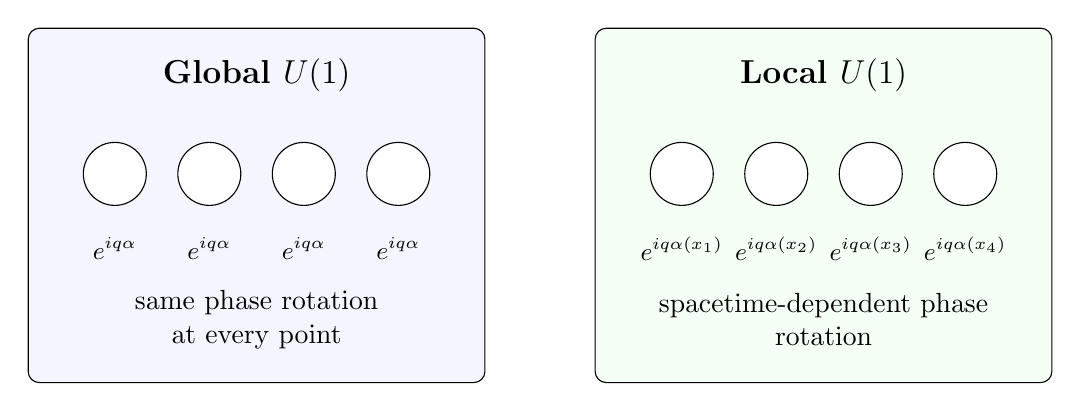
\begin{tikzpicture}[node distance=0.8cm and 1.2cm, arr/.style={-{Latex[length=3mm]}, thick}]
	\node[draw, rounded corners, minimum width=5.8cm, minimum height=4.5cm, align=center, fill=blue!4] (A) at (0,0) {};
	\node[draw, rounded corners, minimum width=5.8cm, minimum height=4.5cm, align=center, fill=green!4] (B) at (7.2,0) {};
	\node[font=\bfseries\large] at (A.north) [yshift=-0.6cm] {Global $U(1)$};
	\node[font=\bfseries\large] at (B.north) [yshift=-0.6cm] {Local $U(1)$};
	\foreach \x/\lbl in {-1.8/$e^{iq\alpha}$,-0.6/$e^{iq\alpha}$,0.6/$e^{iq\alpha}$,1.8/$e^{iq\alpha}$}{
		\node[draw,circle,minimum size=8mm,fill=white] at ($(A.center)+(\x,0.4)$) {};
		\node at ($(A.center)+(\x,-0.55)$) {\small \lbl};}
	\foreach \x/\lbl in {-1.8/$e^{iq\alpha(x_1)}$,-0.6/$e^{iq\alpha(x_2)}$,0.6/$e^{iq\alpha(x_3)}$,1.8/$e^{iq\alpha(x_4)}$}{
		\node[draw,circle,minimum size=8mm,fill=white] at ($(B.center)+(\x,0.4)$) {};
		\node at ($(B.center)+(\x,-0.55)$) {\small \lbl};}
	\node[align=center] at ($(A.center)+(0,-1.45)$) {same phase rotation\\at every point};
	\node[align=center] at ($(B.center)+(0,-1.45)$) {spacetime-dependent phase\\rotation};
\end{tikzpicture}
\caption{Schematic comparison between global and local internal symmetry.}
\label{fig:global-vs-local}
\end{figure}



\end{comment}




\begin{takehomebox}
\vspace{0.25cm}
The failure of the ordinary derivative under a local transformation is the decisive clue of gauge theory. It shows that the free theory cannot realize local symmetry by itself and therefore forces the introduction of a new field and a new derivative operator.
\end{takehomebox}

\begin{guidedchecksbox}
\vspace{0.25cm}
\begin{enumerate}[leftmargin=1.6em,label=\arabic*.]
    \item Starting from \(\psi'(x)=\ee^{\ii q\alpha(x)}\psi(x)\), derive \eqref{eq:ordinary-derivative-local-expanded} step by step.
    \item Show explicitly that the mass term remains invariant even in the local case.
    \item Verify \eqref{eq:kinetic-term-local-obstruction} and identify the current appearing in the extra term.
\end{enumerate}
\end{guidedchecksbox}





\section{Covariant derivative and the emergence of the gauge field}

\subsection{Definition of the covariant derivative}

We seek a modified derivative operator that transforms covariantly under the local symmetry. Motivated by the unwanted term in \eqref{eq:ordinary-derivative-local-expanded}, we introduce a new four-vector field \(A_\mu(x)\) and define
\begin{equation}
D_\mu \equiv \p_\mu-\ii qA_\mu.
\label{eq:abelian-covariant-derivative-expanded}
\end{equation}
The logic of this step is fundamental. The gauge field is not introduced because one already knows the answer from electromagnetism. It is introduced because local covariance requires a compensating structure.

\subsection{Deriving the Abelian gauge-field transformation law}

We now demand that the covariant derivative act on \(\psi\) in such a way that
\begin{equation}
D_\mu'\psi' = \ee^{\ii q\alpha(x)}D_\mu\psi.
\label{eq:covariant-demand-expanded}
\end{equation}
Using
\[
D_\mu' = \p_\mu-\ii qA_\mu',
\qquad
\psi'=\ee^{\ii q\alpha}\psi,
\]
the left-hand side becomes
\begin{align}
D_\mu'\psi'
&=(\p_\mu-\ii qA_\mu')(\ee^{\ii q\alpha}\psi)
\nonumber\\
&=\ee^{\ii q\alpha}\p_\mu\psi+\ii q(\p_\mu\alpha)\ee^{\ii q\alpha}\psi-\ii qA_\mu'\ee^{\ii q\alpha}\psi
\nonumber\\
&=\ee^{\ii q\alpha}\Bigl(\p_\mu\psi+\ii q(\p_\mu\alpha)\psi-\ii qA_\mu'\psi\Bigr).
\end{align}
For this to equal the right-hand side of \eqref{eq:covariant-demand-expanded}, namely
\[
\ee^{\ii q\alpha}(\p_\mu-\ii qA_\mu)\psi,
\]
we must require
\[
A_\mu' = A_\mu+\p_\mu\alpha.
\]
Thus the Abelian gauge field transforms as
\begin{equation}
A_\mu\longrightarrow A_\mu' = A_\mu+\p_\mu\alpha.
\label{eq:abelian-gauge-transform-expanded}
\end{equation}



\subsection{Gauge covariance of \texorpdfstring{$D_\mu\psi$}{Dmu psi}}

Substituting \eqref{eq:abelian-gauge-transform-expanded} back into the transformed covariant derivative, one finds
\begin{align}
D_\mu'\psi'
&=(\p_\mu-\ii qA_\mu')(\ee^{\ii q\alpha}\psi)
\nonumber\\
&=\ee^{\ii q\alpha}\Bigl(\p_\mu\psi+\ii q(\p_\mu\alpha)\psi-\ii q(A_\mu+\p_\mu\alpha)\psi\Bigr)
\nonumber\\
&=\ee^{\ii q\alpha}(\p_\mu-\ii qA_\mu)\psi
\nonumber\\
&=\ee^{\ii q\alpha}D_\mu\psi.
\end{align}
The extra term has been canceled exactly. This is the central algebraic achievement of the gauge principle in the Abelian case.

\subsection{Interpretation: why a gauge field is unavoidable}

The compensation mechanism just derived is often presented as a formal trick, but it is better understood as a structural necessity. The local symmetry transformation introduces a mismatch between neighboring points in spacetime. The gauge field keeps track of how the phase convention changes from point to point and corrects the derivative accordingly. In this sense the covariant derivative plays a role analogous to a connection: it provides a rule for comparing field values at nearby spacetime points in a way compatible with local symmetry.

\begin{definition}{Covariant derivative}{def-covariant-derivative}
Given a matter field \(\psi\) transforming under a local symmetry, the \emph{covariant derivative} is a derivative operator \(D_\mu\) constructed so that \(D_\mu\psi\) transforms in the same way as \(\psi\) itself. In the Abelian case discussed here,
\[
D_\mu=\p_\mu-\ii qA_\mu,
\qquad
A_\mu\to A_\mu+\p_\mu\alpha.
\]
\end{definition}

\begin{remarkbox}{Gauge symmetry and gauge redundancy}{remark-gauge-redundancy}
A gauge transformation usually does not change the underlying physical situation. It changes the field description of that situation. In that sense, gauge symmetry is better thought of as a redundancy of description. But it is a highly constraining redundancy: it dictates which combinations of fields and derivatives are allowed in the Lagrangian and therefore controls the form of the interaction theory.
\end{remarkbox}




\begin{comment}

\begin{figure}[H]
\centering
\begin{tikzpicture}[
	box/.style={rounded corners, draw=black, very thick, align=center, minimum height=1.05cm, text width=4.8cm, fill=blue!4},
	arr/.style={-{Latex[length=3mm]}, very thick}
	]
	\node[box] (p) at (0,0) {$\partial_\mu\psi\ \to\ e^{iq\alpha(x)}\big(\partial_\mu\psi + iq(\partial_\mu\alpha)\psi\big)$};
	\node[box, fill=red!6] (bad) at (0,-2.0) {extra term\\$iq(\partial_\mu\alpha)\psi$};
	\node[box, fill=green!6] (A) at (7.2,0) {$A_\mu\to A_\mu+\partial_\mu\alpha$};
	\node[box, fill=green!10] (D) at (3.6,-4.0) {$D_\mu\psi=(\partial_\mu-iqA_\mu)\psi\\\to e^{iq\alpha(x)}D_\mu\psi$};
	\draw[arr] (p) -- (bad);
	\draw[arr] (A) -- (D);
	\draw[arr] (bad) -- node[above,sloped]{cancelled by gauge-field transformation} (D);
	\draw[arr] (p.east) -- node[above]{repair the derivative} (A.west);
\end{tikzpicture}
\caption{The compensating role of the gauge field in a local \texorpdfstring{$U(1)$}{U(1)} theory.}
\label{fig:gauge-compensation}
\end{figure}

\end{comment}


\begin{takehomebox}
\vspace{0.25cm}
The gauge field is not introduced by guesswork. It is forced upon the theory by the requirement that local symmetry should be realized consistently. The covariant derivative is therefore the first concrete expression of the gauge principle.
\end{takehomebox}




\section{QED as the prototype Abelian gauge theory}

\subsection{From covariance to interaction}

Once the covariant derivative has been constructed, the matter part of the local gauge theory is obtained by the minimal replacement

\[
\p_\mu\longrightarrow D_\mu
\]

in the free Dirac Lagrangian. This gives

\begin{equation}
\Lag_{\text{matter}} = \psibar(\ii\gmu D_\mu-m)\psi.
\label{eq:qed-matter-compact-expanded}
\end{equation}

Expanding the covariant derivative step by step,

\begin{align}
\Lag_{\text{matter}}
&=
\psibar\Bigl(\ii\gmu(\p_\mu-\ii qA_\mu)-m\Bigr)\psi
\nonumber\\
&=
\psibar(\ii\gmu\p_\mu-m)\psi + q\,\psibar\gmu\psi\,A_\mu.
\label{eq:qed-matter-expanded-full}
\end{align}

Thus the interaction term is

\begin{equation}
\Lag_{\text{int}} = + q\,\psibar\gmu\psi\,A_\mu.
\label{eq:qed-interaction-term-expanded}
\end{equation}

If we define the current

\begin{equation}
j^\mu = q\,\psibar\gamma^\mu\psi,
\label{eq:qed-current-expanded}
\end{equation}

then the interaction can be written compactly as

\begin{equation}
\Lag_{\text{int}}= + j^\mu A_\mu.
\label{eq:qed-current-coupling-expanded}
\end{equation}


This is the first complete realization of the gauge principle. The coupling between the matter current and the gauge field has not been invented independently. It is generated automatically when the ordinary derivative is replaced by the covariant derivative.


\begin{examplebox}{Step-by-step expansion of \texorpdfstring{$\psibar(\ii\gamma^\mu D_\mu-m)\psi$}{psi-bar(i gamma D - m) psi}}{example-qed-step-by-step}
Starting from
\[
\Lag=\psibar(\ii\gmu D_\mu-m)\psi,
\qquad D_\mu=\p_\mu-\ii qA_\mu,
\]
we write
\[
\ii\gmu D_\mu=\ii\gmu\p_\mu + q\gmu A_\mu.
\]
Therefore
\[
\Lag = \psibar(\ii\gmu\p_\mu-m)\psi + q\,\psibar\gmu\psi A_\mu.
\]
The current coupling is not an extra assumption. It is the direct consequence of replacing \(\p_\mu\) by \(D_\mu\).
\end{examplebox}



\subsection{The Abelian field strength from the commutator of covariant derivatives}

The gauge field must also possess its own dynamics. In the Abelian theory these dynamics are encoded in the field strength tensor \(F_{\mu\nu}\). It is pedagogically useful to derive this object from the covariant derivative itself rather than introducing it by definition alone. Acting on a field \(\psi\), we compute
\begin{align}
[D_\mu,D_\nu]\psi
&=
(\p_\mu-\ii qA_\mu)(\p_\nu-\ii qA_\nu)\psi
-(\p_\nu-\ii qA_\nu)(\p_\mu-\ii qA_\mu)\psi
\nonumber\\
&=
-\ii q\bigl(\p_\mu A_\nu-\p_\nu A_\mu\bigr)\psi.
\end{align}
This motivates the definition
\begin{equation}
F_{\mu\nu}=\p_\mu A_\nu-\p_\nu A_\mu,
\qquad
[D_\mu,D_\nu]=-\ii qF_{\mu\nu}.
\label{eq:abelian-field-strength-expanded}
\end{equation}
In words, the field strength measures the obstruction to commuting covariant derivatives. In the Abelian case the obstruction is entirely due to the spacetime variation of the gauge field; there is no commutator of gauge fields because ordinary functions commute.



\subsection{Gauge invariance of the Abelian field strength}

Under the Abelian gauge transformation \(A_\mu\to A_\mu+\p_\mu\alpha\), the field strength transforms as
\begin{align}
F'_{\mu\nu}
&=
\p_\mu(A_\nu+\p_\nu\alpha)-\p_\nu(A_\mu+\p_\mu\alpha)
\nonumber\\
&=
\p_\mu A_\nu-\p_\nu A_\mu + \p_\mu\p_\nu\alpha-\p_\nu\p_\mu\alpha
\nonumber\\
&=
F_{\mu\nu},
\end{align}
because ordinary partial derivatives commute. The field strength is therefore gauge invariant. This immediately justifies the gauge-field kinetic term
\begin{equation}
\Lag_{\text{gauge}}=-\frac14 F_{\mu\nu}F^{\mu\nu}.
\label{eq:abelian-gauge-kinetic-expanded}
\end{equation}
Combining matter and gauge sectors, the full QED Lagrangian is
\begin{equation}
\Lag_{\text{QED}}=-\frac14F_{\mu\nu}F^{\mu\nu}+\psibar(\ii\gmu D_\mu-m)\psi.
\label{eq:qed-full-expanded-edition}
\end{equation}



\subsection{An explicit unpacking of \texorpdfstring{$\Lag_{\text{QED}}$}{LQED} and its equations of motion}

The compact form of the QED Lagrangian is pedagogically efficient, but it is useful to unpack it explicitly and then derive its equations of motion. Starting from
\begin{equation}
	\Lag_{\text{QED}}
	=
	-\frac14 F_{\mu\nu}F^{\mu\nu}
	+
	\bar\psi(\ii\gmu D_\mu-m)\psi,
	\qquad
	D_\mu=\p_\mu-\ii qA_\mu,
	\label{eq:LQED-compact-recalled}
\end{equation}
we expand the fermion term step by step:
\begin{align}
	\bar\psi(\ii\gmu D_\mu-m)\psi
	&=
	\bar\psi\Bigl[\ii\gmu(\p_\mu-\ii qA_\mu)-m\Bigr]\psi
	\nonumber\\
	&=
	\bar\psi(\ii\gmu\p_\mu-m)\psi
	+
	q\,\bar\psi\gmu\psi\,A_\mu.
	\label{eq:qed-matter-expansion}
\end{align}
Therefore the expanded QED Lagrangian is
\begin{equation}
	\Lag_{\text{QED}}
	=
	-\frac14 F_{\mu\nu}F^{\mu\nu}
	+
	\bar\psi(\ii\gmu\p_\mu-m)\psi
	+
	q\,\bar\psi\gmu\psi\,A_\mu.
	\label{eq:LQED-expanded}
\end{equation}
It is useful to read this as three pieces:
\begin{equation}
	\Lag_{\text{QED}}
	=
	\underbrace{-\frac14 F_{\mu\nu}F^{\mu\nu}}_{\text{free gauge field}}
	+
	\underbrace{\bar\psi(\ii\gmu\p_\mu-m)\psi}_{\text{free Dirac field}}
	+
	\underbrace{q\,\bar\psi\gmu\psi\,A_\mu}_{\text{matter--gauge interaction}}.
	\label{eq:LQED-three-pieces}
\end{equation}

We may now derive the equations of motion. Varying with respect to \(\bar\psi\) gives the Dirac equation in the presence of the gauge field:
\begin{equation}
	(\ii\gmu D_\mu-m)\psi=0.
	\label{eq:QED-Dirac-eom}
\end{equation}

For the gauge field, we use the Euler--Lagrange equation
\[
\p_\nu\!\left(\frac{\partial \Lag_{\text{QED}}}{\partial(\p_\nu A_\mu)}\right)
-
\frac{\partial \Lag_{\text{QED}}}{\partial A_\mu}
=0.
\]
The required derivatives are
\begin{equation}
	\frac{\partial \Lag_{\text{QED}}}{\partial A_\mu}
	=
	q\,\bar\psi\gmu\psi,
	\qquad
	\frac{\partial \Lag_{\text{QED}}}{\partial(\p_\nu A_\mu)}
	=
	-\,F^{\nu\mu}.
	\label{eq:QED-EL-ingredients}
\end{equation}
Hence the gauge-field equation of motion is
\begin{equation}
	\p_\nu F^{\nu\mu}
	=
	-\,q\,\bar\psi\gmu\psi
	\equiv
	-\,j^\mu,
	\qquad
	j^\mu\equiv q\,\bar\psi\gmu\psi.
	\label{eq:QED-Maxwell-eom}
\end{equation}

With the sign conventions of these notes, the source appears with a minus sign on the right-hand side because the interaction term in the Lagrangian is \(+\,j^\mu A_\mu\). In conventions where the interaction term is written as \(-\,j^\mu A_\mu\), the Maxwell equation is written with the opposite sign.

Taking \(\p_\mu\) of \eqref{eq:QED-Maxwell-eom} and using the antisymmetry of \(F^{\mu\nu}\), one immediately obtains
\begin{equation}
	\p_\mu j^\mu=0.
	\label{eq:QED-current-conservation-from-EOM}
\end{equation}
So the gauge-field equation of motion is automatically consistent with current conservation.

It is also worth noticing that the Abelian gauge-field equation is linear in the gauge field, because
\[
F_{\mu\nu}=\p_\mu A_\nu-\p_\nu A_\mu
\]
contains no quadratic \(AA\) term. This linearity is a special feature of the Abelian theory and will contrast with the Yang--Mills case discussed later.




\begin{remarkbox}{A straightforward multi-species generalization}{remark-qed-multispecies}
For several charged fermion species \(\psi_f\), the expanded Abelian gauge theory takes the form
	\[
	\Lag_{\text{QED}}
	=
	-\frac14 F_{\mu\nu}F^{\mu\nu}
	+
	\sum_f \bar\psi_f(\ii\gmu\p_\mu-m_f)\psi_f
	+
	\sum_f q_f\,\bar\psi_f\gmu\psi_f\,A_\mu.
	\]
For the pedagogical purposes of the present module, however, the one-field form is enough to display the gauge-theory logic cleanly.
\end{remarkbox}



\subsection{A bridge from Maxwell theory to QED}

From a historical and conceptual point of view, QED may be understood as a unification of the relativistic Dirac field with the Maxwell field. The Maxwell field already carries the gauge redundancy
\[
A_\mu\to A_\mu+\p_\mu\alpha,
\]
and the classical electromagnetic field strength is precisely
\[
F_{\mu\nu}=\p_\mu A_\nu-\p_\nu A_\mu.
\]
What the gauge principle adds is a compelling explanation for why the Maxwell field couples to the Dirac current in the way it does. The source term in Maxwell's equations is not inserted independently; it arises from local covariance of the matter field. In this sense, QED is the quantum-field-theoretic completion of the classical idea that a conserved electric current couples to the electromagnetic field.



\subsection{Why the photon is massless at this stage}

At the level of the Abelian gauge theory constructed here, the gauge field is massless. The reason is structural. A term of the form
\begin{equation}
\frac12 m_A^2 A_\mu A^\mu
\label{eq:mass-term-abelian}
\end{equation}
is not invariant under
\[
A_\mu\to A_\mu+\p_\mu\alpha.
\]
Indeed,
\[
A_\mu A^\mu \to (A_\mu+\p_\mu\alpha)(A^\mu+\p^\mu\alpha),
\]
which produces extra terms that do not cancel. Therefore the local \(U(1)\) symmetry forbids an explicit mass term for the gauge field. The photon is massless in QED precisely because the local gauge symmetry is unbroken.

\begin{remarkbox}{Why \texorpdfstring{$A_\mu A^\mu$}{AμAμ} is forbidden}{remark-A2-forbidden}
The term \(A_\mu A^\mu\) is Lorentz invariant, but that is not enough. In gauge theory one must satisfy both Lorentz covariance and local gauge invariance. Since \(A_\mu A^\mu\) is not invariant under \(A_\mu\to A_\mu+\p_\mu\alpha\), it is forbidden in the unbroken Abelian theory.
\end{remarkbox}



\subsection{Gauge symmetry, current conservation, and physical meaning}

With the convention
\[
D_\mu = \partial_\mu - i q A_\mu
\]
used in these notes, the QED interaction term is written as
\[
\mathcal{L}_{\text{int}} = + j^\mu A_\mu,
\]
where
\[
j^\mu = q\,\bar{\psi}\gamma^\mu\psi.
\]



This makes the relationship between current conservation and gauge invariance especially transparent, but the precise statement should be made carefully. For an \emph{external} source coupling of the form \(j^\mu A_\mu\), gauge invariance of the action requires the source to be conserved, \( \partial_\mu j^\mu = 0 \). In dynamical QED, however, the matter--gauge interaction is not introduced as an arbitrary external source term; it arises directly from the gauge-covariant Dirac Lagrangian \( \bar{\psi}(i\gamma^\mu D_\mu - m)\psi \). In that sense, local gauge invariance and current conservation are closely related, but not in exactly the same way as for a prescribed classical source. The conserved \(U(1)\) current that first appeared in the global symmetry analysis of Section~2 is precisely the matter current that couples to the gauge field in the local theory.


It is also useful to keep the more conceptual viewpoint in mind. Gauge symmetry is often best thought of as gauge redundancy. The point is not that nature is physically invariant under arbitrary changes of gauge description in the same way that a crystal might be invariant under a geometric rotation. Rather, the field description contains unphysical redundancy, and the redundancy constrains the admissible Lagrangian. That is why local symmetry is so powerful even when interpreted as a redundancy.




\begin{figure}[H]
\centering
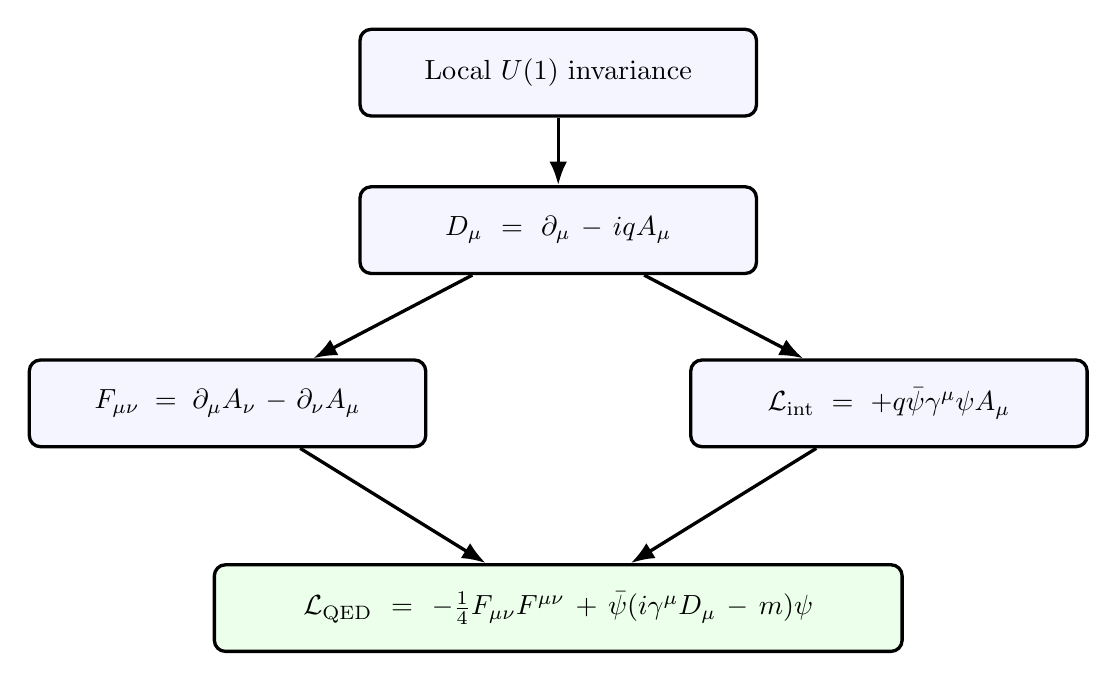
\begin{tikzpicture}[
	block/.style={rounded corners, draw=black, very thick, align=center, minimum height=1.1cm, text width=4.8cm, fill=blue!4},
	arr/.style={-{Latex[length=3mm]}, very thick}
	]
	\node[block] (g) at (0,0) {Local $U(1)$ invariance};
	\node[block] (d) at (0,-2.0) {$D_\mu=\partial_\mu-iqA_\mu$};
	\node[block] (f) at (-4.2,-4.2) {$F_{\mu\nu}=\partial_\mu A_\nu-\partial_\nu A_\mu$};
	\node[block] (i) at (4.2,-4.2) {$\mathcal L_{\rm int}=+q\bar\psi\gamma^\mu\psi A_\mu$};
	\node[block, fill=green!8, text width=8.5cm] (L) at (0,-6.8) {$\mathcal L_{\rm QED}=-\frac14F_{\mu\nu}F^{\mu\nu}+\bar\psi(i\gamma^\mu D_\mu-m)\psi$};
	\draw[arr] (g) -- (d);
	\draw[arr] (d) -- (f);
	\draw[arr] (d) -- (i);
	\draw[arr] (f) -- (L);
	\draw[arr] (i) -- (L);
\end{tikzpicture}
\caption{QED as the first complete local gauge theory.}
\label{fig:qed-structure-expanded}
\end{figure}




\begin{takehomebox}
\vspace{0.25cm}
QED is the prototype gauge theory because the entire gauge-theoretic logic can be seen in closed form. The gauge field, the interaction term, and the field strength all arise because local covariance forces the theory to be written in terms of the covariant derivative.
\end{takehomebox}

\begin{guidedchecksbox}
\vspace{0.25cm}
\begin{enumerate}[leftmargin=1.6em,label=\arabic*.]
    \item Expand \(\psibar(\ii\gmu D_\mu-m)\psi\) carefully and recover the current coupling.
    \item Derive \([D_\mu,D_\nu]=-\ii qF_{\mu\nu}\) explicitly in the Abelian case.
    \item Verify that \(F_{\mu\nu}\) is invariant under \(A_\mu\to A_\mu+\p_\mu\alpha\).
    \item Explain in one sentence why a photon mass term \(A_\mu A^\mu\) is forbidden before symmetry breaking.
\end{enumerate}
\end{guidedchecksbox}




\section{Why QED is not enough: toward non-Abelian symmetry}


\subsection{The limitation of a single Abelian gauge factor}

Quantum electrodynamics is a complete and internally consistent local gauge theory, but it is not enough to describe the full structure of known particle interactions. The Standard Model does not consist of a single \(U(1)\) factor. Instead, its gauge structure is
{\color{red}\[
\SMgauge,
\]}
which contains two non-Abelian factors in addition to the Abelian one. Thus the gauge principle must be generalized beyond a single commuting phase symmetry.

The Abelian theory already teaches the core lesson: local symmetry forces the introduction of gauge fields and interaction terms. But its simplicity depends crucially on the fact that the group elements commute. Once one moves to a symmetry with non-commuting generators, the theory changes qualitatively. Matter fields naturally come in multiplets, gauge fields become Lie-algebra valued, and the gauge bosons themselves can interact.

\subsection{Groups versus algebras}

A continuous symmetry group is most efficiently studied near the identity. If \(U\in G\) is close to the identity, one may write
\begin{equation}
U=\ee^{\ii\alpha^aT^a}=\mathbf{1}+\ii\alpha^aT^a+\mc{O}(\alpha^2),
\label{eq:group-element-near-identity}
\end{equation}
where the \(T^a\) are the generators. The collection of generators together with their commutation relations defines the Lie algebra of the group. For our purposes, the Lie algebra is the more directly useful object because it controls infinitesimal transformations and appears explicitly in the covariant derivative.

The commutators of the generators take the form
\begin{equation}
\comm{T^a}{T^b}=\ii f^{abc}T^c,
\label{eq:lie-algebra-commutator-expanded}
\end{equation}
where \(f^{abc}\) are the structure constants. If all structure constants vanish, the algebra is Abelian. If not, it is non-Abelian. In that sense, the passage from QED to Yang--Mills theory is the passage from a commuting algebra to a non-commuting one.

\subsection{Generators, infinitesimal transformations, and representations}

Suppose \(\psi\) is a field multiplet transforming in some representation \(R\) of the group. Then an infinitesimal transformation is written as
\begin{equation}
\psi\to \psi'=(\mathbf{1}+\ii\alpha^aT^a_R)\psi,
\label{eq:infinitesimal-transformation-rep}
\end{equation}
where \(T^a_R\) denotes the matrix representation of the generator on the multiplet. This already shows why the language of representation theory is unavoidable: to know how a field transforms is to know which matrices represent the generators on that field.

A singlet, doublet, or triplet is therefore not a decorative label. It is a statement about the dimension and transformation law of the field under the symmetry group. This will matter enormously in the Standard Model, where left-chiral fermions arrange themselves into weak doublets, right-chiral fermions are weak singlets, and quarks transform as color triplets.

\subsection{Fundamental and adjoint representations}

Two representations are especially important for gauge theory. The first is the \emph{fundamental representation}, which is usually the one carried by the matter fields. For \(\SU(2)\), the fundamental representation is two-dimensional, and the generators are conveniently written as
\begin{equation}
T^i = \frac{\tau^i}{2},
\label{eq:su2-fund-generators}
\end{equation}
with \(\tau^i\) the Pauli matrices. For \(\SU(3)\), the fundamental representation is three-dimensional, and the generators are commonly taken as
\begin{equation}
T^a=\frac{\lambda^a}{2},
\label{eq:su3-fund-generators}
\end{equation}
with \(\lambda^a\) the Gell--Mann matrices.

The second is the \emph{adjoint representation}. In this representation the generators act on the Lie algebra itself. Gauge fields live naturally in this representation because they carry a Lie-algebra index \(a\). This is why gluons come in an octet of color and why the weak gauge bosons form a triplet before electroweak symmetry breaking.




\subsection{A concrete \texorpdfstring{$SU(2)$}{SU(2)} example}

For \(\SU(2)\), the Pauli matrices satisfy
\[
\comm{\tau^i}{\tau^j}=2\ii\epsilon^{ijk}\tau^k.
\]
Therefore the normalized generators \(T^i=\tau^i/2\) obey
\begin{equation}
\comm{T^i}{T^j}=\ii\epsilon^{ijk}T^k.
\label{eq:su2-algebra-expanded}
\end{equation}
This example is pedagogically ideal because it is both familiar and nontrivial. The algebra is already non-Abelian, so it exhibits exactly the structural difference that later appears in the weak interaction sector of the Standard Model.



\subsection{An orientation-level remark on \texorpdfstring{$SU(3)$}{SU(3)}}

The group \(\SU(3)\) is structurally similar but larger. It has eight generators and therefore eight gauge bosons in the adjoint representation. The full phenomenology of \(\SU(3)_c\) belongs to QCD and will be studied later, but it is useful already now to note that the color gauge sector is a direct non-Abelian generalization of the Yang--Mills logic developed here. The fact that \(\SU(3)\) is non-Abelian implies, already at the formal level, that the gluons carry color charge and self-interact.



\subsection{Why non-commutativity is physically decisive}

At first sight, the difference between Abelian and non-Abelian symmetry may look like a technical matter of whether generators commute. In reality, it is one of the most consequential structural differences in all of gauge theory. Once the commutator of generators is nonzero, the gauge field must be treated as Lie-algebra valued and the field strength acquires a commutator term. That term leads to self-interactions of the gauge bosons. In other words, non-commutativity is what makes Yang--Mills theory qualitatively richer than Maxwell theory.

\begin{definition}{Lie algebra and structure constants}{def-lie-algebra-expanded}
Given a continuous Lie group, the generators of infinitesimal transformations satisfy commutation relations
\[
\comm{T^a}{T^b}=\ii f^{abc}T^c.
\]
The coefficients \(f^{abc}\) are called the \emph{structure constants}. If all such commutators vanish, the group is Abelian. If they do not, the group is non-Abelian.
\end{definition}


\begin{remarkbox}{Representations are transformation rules}{remark-representations-expanded}
When we say that a field is a singlet, doublet, triplet, or more generally belongs to a certain representation, we are specifying how the generators act on that field. This determines which matrices appear in the covariant derivative and therefore which gauge interactions the field experiences.
\end{remarkbox}



\begin{comment}

\begin{figure}[H]
\centering
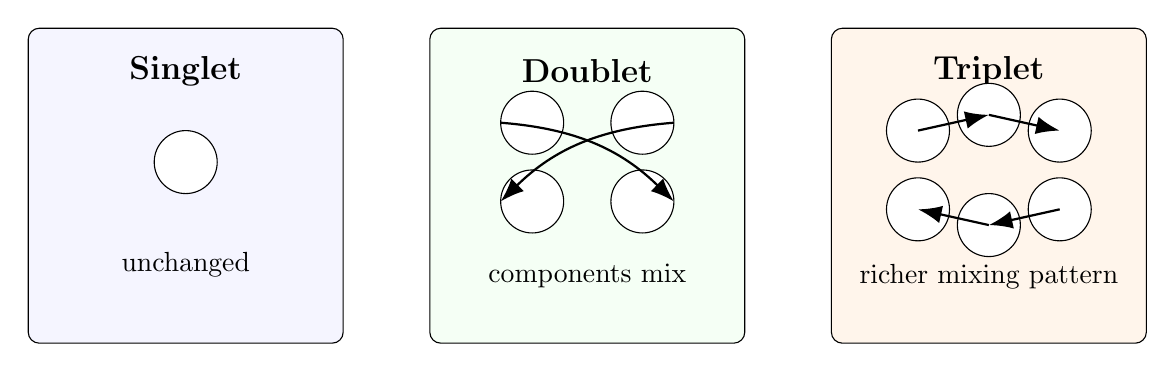
\begin{tikzpicture}[arr/.style={-{Latex[length=3mm]}, thick}]
	\node[draw, rounded corners, fill=blue!4, minimum width=4cm, minimum height=4cm] (S) at (0,0) {};
	\node[draw, rounded corners, fill=green!4, minimum width=4cm, minimum height=4cm] (D) at (5.1,0) {};
	\node[draw, rounded corners, fill=orange!8, minimum width=4cm, minimum height=4cm] (T) at (10.2,0) {};
	\node[font=\bfseries\large] at ($(S.north)+(0,-0.55)$) {Singlet};
	\node[font=\bfseries\large] at ($(D.north)+(0,-0.55)$) {Doublet};
	\node[font=\bfseries\large] at ($(T.north)+(0,-0.55)$) {Triplet};
	\node[draw,circle,minimum size=8mm,fill=white] at ($(S.center)+(0,0.3)$) {};
	\node at ($(S.center)+(0,-1.0)$) {unchanged};
	\foreach \y in {0.8,-0.2}{\node[draw,circle,minimum size=8mm,fill=white] at ($(D.center)+(-0.7,\y)$) {};
		\node[draw,circle,minimum size=8mm,fill=white] at ($(D.center)+(0.7,\y)$) {};}
	\draw[arr] ($(D.center)+(-1.1,0.8)$) to[bend left=20] ($(D.center)+(1.1,-0.2)$);
	\draw[arr] ($(D.center)+(1.1,0.8)$) to[bend right=20] ($(D.center)+(-1.1,-0.2)$);
	\foreach \x/\y in {-0.9/0.7,0/0.9,0.9/0.7}{\node[draw,circle,minimum size=8mm,fill=white] at ($(T.center)+(\x,\y)$) {};}
	\foreach \x/\y in {-0.9/-0.3,0/-0.5,0.9/-0.3}{\node[draw,circle,minimum size=8mm,fill=white] at ($(T.center)+(\x,\y)$) {};}
	\draw[arr] ($(T.center)+(-0.9,0.7)$) -- ($(T.center)+(0,0.9)$);
	\draw[arr] ($(T.center)+(0,0.9)$) -- ($(T.center)+(0.9,0.7)$);
	\draw[arr] ($(T.center)+(0.9,-0.3)$) -- ($(T.center)+(0,-0.5)$);
	\draw[arr] ($(T.center)+(0,-0.5)$) -- ($(T.center)+(-0.9,-0.3)$);
	\node[align=center] at ($(D.center)+(0,-1.15)$) {components mix};
	\node[align=center] at ($(T.center)+(0,-1.15)$) {richer mixing pattern};
\end{tikzpicture}
\caption{Multiplets and representations as transformation rules.}
\label{fig:multiplets-and-reps}
\end{figure}


\end{comment}
	
	


\begin{takehomebox}
\vspace{0.25cm}
The move from Abelian to non-Abelian symmetry is not just the replacement of one group by another. It introduces a qualitatively new structure: matrix-valued transformations, Lie-algebra-valued gauge fields, and non-commuting generators whose commutator will later reappear directly in the field strength tensor.
\end{takehomebox}




\section{Non-Abelian gauge symmetry and Yang--Mills theory}

\subsection{Matter fields in a multiplet}

Let \(\psi(x)\) denote a column vector of fields transforming in some representation \(R\) of a Lie group \(G\). A local transformation acts as
\begin{equation}
\psi(x)\to \psi'(x)=U(x)\psi(x),
\qquad
U(x)=\ee^{\ii\alpha^a(x)T^a}.
\label{eq:local-multiplet-transform-expanded}
\end{equation}
Exactly as in the Abelian case, the ordinary derivative fails to transform covariantly once \(\alpha^a\) depends on spacetime. The remedy is again to introduce a covariant derivative, but now the gauge field must carry the generator structure of the group itself.

\subsection{Why a Lie-algebra-valued gauge field is natural}

The local transformation acts by a matrix \(U(x)\). Therefore the compensating field must also be an object that can live in the same internal space. This motivates the definition
\begin{equation}
A_\mu(x)=A_\mu^a(x)T^a.
\label{eq:lie-algebra-valued-gauge-field}
\end{equation}
The gauge field is thus not a single ordinary vector field but a Lie-algebra-valued one. This is a natural generalization of the Abelian case: in \(U(1)\), the single generator is effectively just a number, so one can suppress the matrix structure. In a non-Abelian theory the generator structure is essential and cannot be hidden.

\subsection{Non-Abelian covariant derivative}

The covariant derivative is defined by
\begin{equation}
D_\mu = \p_\mu-\ii gA_\mu,
\label{eq:nonabelian-covariant-derivative-expanded}
\end{equation}
where \(A_\mu=A_\mu^aT^a\). The defining covariance condition is
\begin{equation}
D_\mu'\psi' = U(D_\mu\psi).
\label{eq:nonabelian-covariance-demand}
\end{equation}
This is the exact non-Abelian analog of the Abelian requirement that \(D_\mu\psi\) transform in the same way as \(\psi\) itself.

\subsection{Gauge transformation law of the non-Abelian gauge field}

Demanding \eqref{eq:nonabelian-covariance-demand} fixes the transformation law of the gauge field. Starting from
\[
(\p_\mu-\ii gA_\mu')U\psi = U(\p_\mu-\ii gA_\mu)\psi,
\]
and rearranging, one obtains
\begin{equation}
A_\mu' = U A_\mu U^{-1} + \frac{\ii}{g}(\p_\mu U)U^{-1}.
\label{eq:nonabelian-gauge-transform-expanded}
\end{equation}
This formula is already much richer than the Abelian one because the gauge field appears on both sides multiplied by the group element. For infinitesimal transformations, writing
\[
U=\mathbf{1}+\ii\alpha+\mc{O}(\alpha^2),
\qquad \alpha=\alpha^aT^a,
\]
one finds
\begin{equation}
\delta A_\mu = \p_\mu\alpha - \ii g\comm{A_\mu}{\alpha}.
\label{eq:nonabelian-gauge-variation-expanded}
\end{equation}
In component form this becomes
\begin{equation}
\delta A_\mu^a = \p_\mu\alpha^a + g f^{abc}\alpha^b A_\mu^c.
\label{eq:nonabelian-gauge-variation-components}
\end{equation}



\subsection{Field strength from the commutator \texorpdfstring{$[D_\mu,D_\nu]$}{[Dmu,Dnu]}}

The field strength is once again derived from the commutator of covariant derivatives:
\begin{align}
[D_\mu,D_\nu]
&=
[\p_\mu-\ii gA_\mu,\p_\nu-\ii gA_\nu]
\nonumber\\
&=
-\ii g(\p_\mu A_\nu-\p_\nu A_\mu)-g^2\comm{A_\mu}{A_\nu}.
\end{align}
This motivates the definition
\begin{equation}
F_{\mu\nu}=\p_\mu A_\nu-\p_\nu A_\mu-\ii g\comm{A_\mu}{A_\nu},
\qquad
[D_\mu,D_\nu]=-\ii gF_{\mu\nu}.
\label{eq:nonabelian-field-strength-expanded}
\end{equation}
This is the central formula of Yang--Mills theory. Compared with the Abelian case, the new term is the commutator of the gauge fields themselves.

\subsection{Component form of the field strength}

To make the structure constants visible, substitute \(A_\mu=A_\mu^aT^a\) into \eqref{eq:nonabelian-field-strength-expanded}:
\begin{align}
F_{\mu\nu}
&=
\bigl(\p_\mu A_\nu^a-\p_\nu A_\mu^a\bigr)T^a
-\ii g A_\mu^aA_\nu^b\comm{T^a}{T^b}
\nonumber\\
&=
\bigl(\p_\mu A_\nu^a-\p_\nu A_\mu^a\bigr)T^a
+gA_\mu^aA_\nu^b f^{abc}T^c.
\end{align}
Relabeling the Lie-algebra index, we obtain
\begin{equation}
F_{\mu\nu}^a = \p_\mu A_\nu^a-\p_\nu A_\mu^a+g f^{abc}A_\mu^bA_\nu^c.
\label{eq:field-strength-components-expanded}
\end{equation}

This is the form in which the Yang--Mills field strength most often appears in applications.  
Unlike the Abelian field strength, the non-Abelian field strength is not itself gauge invariant. Rather, it transforms covariantly:
\begin{equation}
	F'_{\mu\nu} = U F_{\mu\nu} U^{-1}.
\end{equation}
For an infinitesimal transformation \(U = 1 + i\alpha + \mathcal{O}(\alpha^2)\), one correspondingly has
\begin{equation}
	\delta F_{\mu\nu} = i[\alpha, F_{\mu\nu}] .
\end{equation}
This is why gauge-invariant quantities in Yang--Mills theory are built from traces such as \(\mathrm{Tr}(F_{\mu\nu}F^{\mu\nu})\), rather than from the matrix-valued field strength itself.



\begin{examplebox}{Deriving the component form of \texorpdfstring{$F_{\mu\nu}^a$}{Fmunua}}{example-field-strength-components}
Using
\[
A_\mu=A_\mu^aT^a,
\qquad
\comm{T^a}{T^b}=\ii f^{abc}T^c,
\]
we find
\[
-\ii g\comm{A_\mu}{A_\nu} = -\ii gA_\mu^aA_\nu^b\comm{T^a}{T^b}
= gA_\mu^aA_\nu^b f^{abc}T^c.
\]
Combining this with \(\p_\mu A_\nu-\p_\nu A_\mu\) yields
\[
F_{\mu\nu}^a=\p_\mu A_\nu^a-\p_\nu A_\mu^a+g f^{abc}A_\mu^bA_\nu^c.
\]
\end{examplebox}



\subsection{A side-by-side Abelian versus non-Abelian comparison}

It is useful to pause and compare the two structures explicitly:
\begin{align*}
\text{Abelian:}
&\qquad D_\mu=\p_\mu-\ii qA_\mu,
\qquad F_{\mu\nu}=\p_\mu A_\nu-\p_\nu A_\mu,
\\[0.4em]
\text{Non-Abelian:}
&\qquad D_\mu=\p_\mu-\ii gA_\mu,
\qquad F_{\mu\nu}=\p_\mu A_\nu-\p_\nu A_\mu-\ii g\comm{A_\mu}{A_\nu}.
\end{align*}
The difference lies entirely in the commutator. In the Abelian case, the gauge field behaves like an ordinary field and the field strength is linear in \(A_\mu\). In the non-Abelian case, the non-commuting generator structure produces a term quadratic in the gauge fields.



\subsection{Yang--Mills Lagrangian and self-interactions}

The gauge kinetic term of the non-Abelian theory is the Yang--Mills Lagrangian,
\begin{equation}
\Lag_{\text{YM}}=-\frac14 F_{\mu\nu}^aF^{a\mu\nu}
=-\frac12\Tr(F_{\mu\nu}F^{\mu\nu}).
\label{eq:yang-mills-lagrangian-expanded}
\end{equation}
Substituting \eqref{eq:field-strength-components-expanded} into this expression yields schematically
\[
\Lag_{\text{YM}}\sim (\p A)^2 + g(\p A)AA + g^2AAAA.
\]
The first term describes propagation, while the second and third describe triple and quartic gauge-boson interactions. This is the key qualitative difference between Abelian and non-Abelian gauge theory: the gauge bosons themselves carry the charge of the symmetry and therefore interact with one another.



\subsection{A worked \texorpdfstring{$SU(2)$}{SU(2)} example}

For \(\SU(2)\), the structure constants are \(f^{ijk}=\epsilon^{ijk}\). The field strength is therefore
\begin{equation}
W_{\mu\nu}^i=\p_\mu W_\nu^i-\p_\nu W_\mu^i+g\epsilon^{ijk}W_\mu^jW_\nu^k.
\label{eq:su2-field-strength-worked}
\end{equation}
This is exactly the structure that later appears in the electroweak sector of the Standard Model before symmetry breaking. Even before one studies the physical \(W^\pm\) and \(Z\) bosons, the Yang--Mills structure already tells us that the weak gauge fields cannot behave like three independent copies of electrodynamics. Their non-Abelian symmetry ties them together and introduces self-interactions.


\subsection{Why this prepares the way for QCD and electroweak theory}

The Yang--Mills construction is the bridge between the abstract gauge principle and the actual Standard Model. The strong interaction sector is a Yang--Mills theory based on \(\SUc\), while the weak sector before symmetry breaking is a Yang--Mills theory based on \(\SUw\). Thus the conceptual work done here is not an optional mathematical interlude. It is precisely what allows the Standard Model gauge structure to be written down coherently.




%	
%------------------------------------------------
%
\begin{figure}[H]
\centering
\includegraphics[width=0.65\textwidth]{thomson_figF1_triple_quartic_gauge_vertices.jpg}
%\vspace{-6cm}
\begin{center}
\caption{ \small 
Triple and quartic gauge-boson self-interactions in a non-Abelian gauge theory.}
\label{fig:triple_and_quartic_gauge_boson_vertices}
\end{center}
\end{figure} 
%	
%------------------------------------------------
% 


\begin{takehomebox}
\vspace{0.25cm}
The gauge principle survives the move from Abelian to non-Abelian symmetry, but the theory changes qualitatively. The gauge field becomes Lie-algebra valued, the field strength acquires a commutator term, and the gauge bosons themselves necessarily self-interact.
\end{takehomebox}



\begin{guidedchecksbox}
\vspace{0.25cm}
\begin{enumerate}[leftmargin=1.6em,label=\arabic*.]
    \item Starting from \(A_\mu=A_\mu^aT^a\), derive the component form \eqref{eq:field-strength-components-expanded}.
    \item Compare the Abelian and non-Abelian field strengths and identify the precise new term.
    \item For \(\SU(2)\), verify \eqref{eq:su2-algebra-expanded} using the Pauli matrices.
    \item Explain why the presence of the commutator term implies gauge-boson self-interactions.
\end{enumerate}
\end{guidedchecksbox}



\section{From Yang--Mills theory to the Standard Model gauge structure}

\subsection{The guiding equation of the Standard Model}

Having developed the general framework of local gauge theory, we can now specialize to the Standard Model. Its gauge sector is organized by the direct-product group
\begin{equation}
{\color{red}G_{\text{SM}}=\SMgauge.}
\label{eq:sm-gauge-group-expanded}
\end{equation}
This compact equation is one of the central organizing formulas of modern particle physics. It says that the Standard Model is built from three local symmetry factors rather than from a single unified gauge field. Each factor contributes a different part of the observed interaction structure.



\subsection{Physical meaning of the three gauge factors}

The factor \(\SUc\) is the gauge symmetry of color. It acts on quarks and is associated with eight gauge bosons, the gluons. The factor \(\SUw\) is weak isospin. It acts nontrivially on left-chiral fermion doublets and is associated with three gauge fields. The factor \(\UY\) is weak hypercharge, an Abelian symmetry that acts through the hypercharge number \(Y\) carried by each field.

At this stage it is essential to remember that the Standard Model \(U(1)\) factor is \emph{not} yet electromagnetism. Electromagnetism emerges only after electroweak symmetry breaking as the unbroken combination of neutral electroweak gauge fields. In the present module we work in the unbroken phase, where the relevant gauge fields are \(G_\mu^a\), \(W_\mu^i\), and \(B_\mu\).

\begin{remarkbox}{Hypercharge is not yet electromagnetism}{remark-hypercharge-not-em-expanded}
The \(U(1)\) factor in the Standard Model is \(U(1)_Y\), not yet the observed electromagnetic \(U(1)\). The photon appears only after electroweak symmetry breaking. Module~3 therefore focuses on the gauge structure before that breaking occurs.
\end{remarkbox}



\begin{figure}[H]
\centering
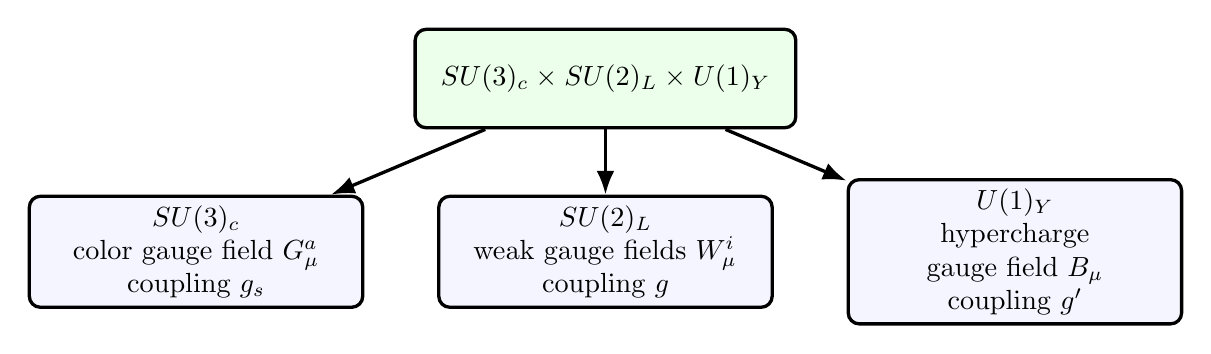
\begin{tikzpicture}[
		block/.style={rounded corners, draw=black, very thick, align=center, minimum height=1.25cm, text width=4.0cm, fill=blue!4}
		]
		\node[block, fill=green!8, text width=4.6cm] (sm) at (0,2.2) {$SU(3)_c\times SU(2)_L\times U(1)_Y$};
		\node[block] (c) at (-5.2,0) {$SU(3)_c$\\color gauge field $G_\mu^a$\\coupling $g_s$};
		\node[block] (w) at (0,0) {$SU(2)_L$\\weak gauge fields $W_\mu^i$\\coupling $g$};
		\node[block] (y) at (5.2,0) {$U(1)_Y$\\hypercharge gauge field $B_\mu$\\coupling $g'$};
		\draw[-{Latex[length=3mm]}, very thick] (sm) -- (c);
		\draw[-{Latex[length=3mm]}, very thick] (sm) -- (w);
		\draw[-{Latex[length=3mm]}, very thick] (sm) -- (y);
\end{tikzpicture}
\caption{Gauge structure of the Standard Model before electroweak symmetry breaking.}
\label{fig:sm-gauge-structure-expanded}
\end{figure}




\begin{takehomebox}
\vspace{0.25cm}
The equation {\color{red}\(\SMgauge\)} is not a mnemonic label for the Standard Model. It is the compact structural statement from which the broad pattern of gauge interactions follows.
\end{takehomebox}






\subsection{Direct-product structure and independent couplings}

Each gauge factor comes with its own gauge field and its own coupling constant:
\[
G_\mu^a\ (a=1,\dots,8),
\qquad
W_\mu^i\ (i=1,2,3),
\qquad
B_\mu,
\]
with couplings
\[
g_s,
\qquad g,
\qquad g'.
\]
A matter field may couple to one, two, or all three sectors depending on which representations it carries. This is one of the cleanest ways to see that the interaction pattern of the Standard Model is encoded in representation theory.







\section{Matter content of one Standard Model generation}

\subsection{Why one generation is the right pedagogical starting point}

The Standard Model contains three generations of quarks and leptons, but from the viewpoint of gauge symmetry all three generations follow the same representation pattern. Their masses and flavor mixing differ, but their gauge transformation properties do not. A single generation therefore already reveals the structure that matters for Module~3.



\subsection{Left-chiral weak doublets}

The left-chiral quarks of one generation are grouped into the weak doublet
\begin{equation}
Q_L=\begin{pmatrix}u_L\\ d_L\end{pmatrix},
\label{eq:QL-doublet-expanded}
\end{equation}
while the left-chiral leptons are grouped into
\begin{equation}
L_L=\begin{pmatrix}\nu_L\\ e_L\end{pmatrix}.
\label{eq:LL-doublet-expanded}
\end{equation}
These are weak doublets because \(\SUw\) acts nontrivially on them. The quark doublet also carries color and is therefore a triplet under \(\SUc\). The lepton doublet is color neutral.




\subsection{Right-chiral weak singlets}

The right-chiral fermions do not form weak doublets in the Standard Model. Instead, they appear as weak singlets:

In the minimal Standard Model, the right-chiral weak singlets are
\(u_R\), \(d_R\), and \(e_R\), while \(\nu_R\) is absent.


The absence of a right-chiral neutrino in the minimal version of the Standard Model is itself a structural statement about field content, though extended models often include such a field. For the purposes of Module~3 we keep the minimal assignment.




\subsection{One-generation representation table}

Using the hypercharge convention \(Q=T_3+Y\), one generation of Standard Model fermions may be summarized as follows:



\begin{table}[H]
\centering
\caption{One-generation fermion content of the Standard Model.}
\label{tab:one-generation-clean}
\begin{tabular}{>{\raggedright\arraybackslash}p{0.18\textwidth}>{\raggedright\arraybackslash}p{0.26\textwidth}>{\centering\arraybackslash}p{0.17\textwidth}>{\centering\arraybackslash}p{0.16\textwidth}>{\centering\arraybackslash}p{0.12\textwidth}}
\toprule
Field & Explicit form & \(\SUc\) & \(\SUw\) & \(Y\) \\
\midrule
\(Q_L\) & \(\begin{pmatrix}u_L\\ d_L\end{pmatrix}\) & \(\mathbf{3}\) & \(\mathbf{2}\) & \(\phantom{-}\frac16\) \\
\(L_L\) & \(\begin{pmatrix}\nu_L\\ e_L\end{pmatrix}\) & \(\mathbf{1}\) & \(\mathbf{2}\) & \(-\frac12\) \\
\(u_R\) & up-type quark singlet & \(\mathbf{3}\) & \(\mathbf{1}\) & \(\phantom{-}\frac23\) \\
\(d_R\) & down-type quark singlet & \(\mathbf{3}\) & \(\mathbf{1}\) & \(-\frac13\) \\
\(e_R\) & charged-lepton singlet & \(\mathbf{1}\) & \(\mathbf{1}\) & \(-1\) \\
\bottomrule
\end{tabular}
\end{table}



In the compact notation commonly used in particle theory, the one-generation assignments are often summarized as
\[
\begin{aligned}
Q_L & : (\mathbf{3},\mathbf{2})_{1/6},
&
L_L & : (\mathbf{1},\mathbf{2})_{-1/2},
\\[0.2em]u_R & : (\mathbf{3},\mathbf{1})_{2/3},
&d_R & : (\mathbf{3},\mathbf{1})_{-1/3},
\\[0.2em]e_R & : (\mathbf{1},\mathbf{1})_{-1}.
\end{aligned}
\]
In the minimal Standard Model no right-handed neutrino is included, although such a field is often added in extensions of the theory. The repeated pattern across the three generations means that, for the purposes of gauge symmetry, one generation is enough to exhibit the full interaction structure.



\subsection{Chirality and the electroweak pattern}

The electroweak sector is chiral because left- and right-chiral fermions transform differently under the gauge group. Chirality is defined through the projectors
\[
\PL=\frac{1-\gfive}{2},
\qquad
\PR=\frac{1+\gfive}{2},
\]
so that \(\psi_L=\PL\psi\) and \(\psi_R=\PR\psi\). In the massless limit, chirality coincides with helicity, but conceptually the two notions are distinct. For the Standard Model, the crucial fact is that the gauge representation depends on chirality: \(Q_L\) and \(L_L\) are weak doublets, whereas \(u_R\), \(d_R\), and \(e_R\) are weak singlets.

This left-right asymmetry is not cosmetic. It is one of the defining reasons why the Standard Model is a chiral gauge theory and why weak interactions violate parity.

\begin{definition}{Chiral gauge theory}{def-chiral-gauge-theory-expanded}
A gauge theory is called \emph{chiral} if left- and right-chiral fermion fields transform differently under the gauge group. The Standard Model is chiral because \(\SUw\) acts nontrivially only on left-chiral fermion doublets, while the right-chiral fermions are weak singlets.
\end{definition}

\begin{remarkbox}{Representations determine interactions}{remark-reps-determine-couplings-expanded}
The assignments \((\mathbf{3},\mathbf{2})_{1/6}\), \((\mathbf{1},\mathbf{2})_{-1/2}\), and so on are not bookkeeping labels. They specify how each field transforms and therefore determine which gauge fields appear in its covariant derivative. In this sense, the representation content already contains the interaction structure.
\end{remarkbox}



\begin{comment}
	
\begin{figure}[H]
	\centering
	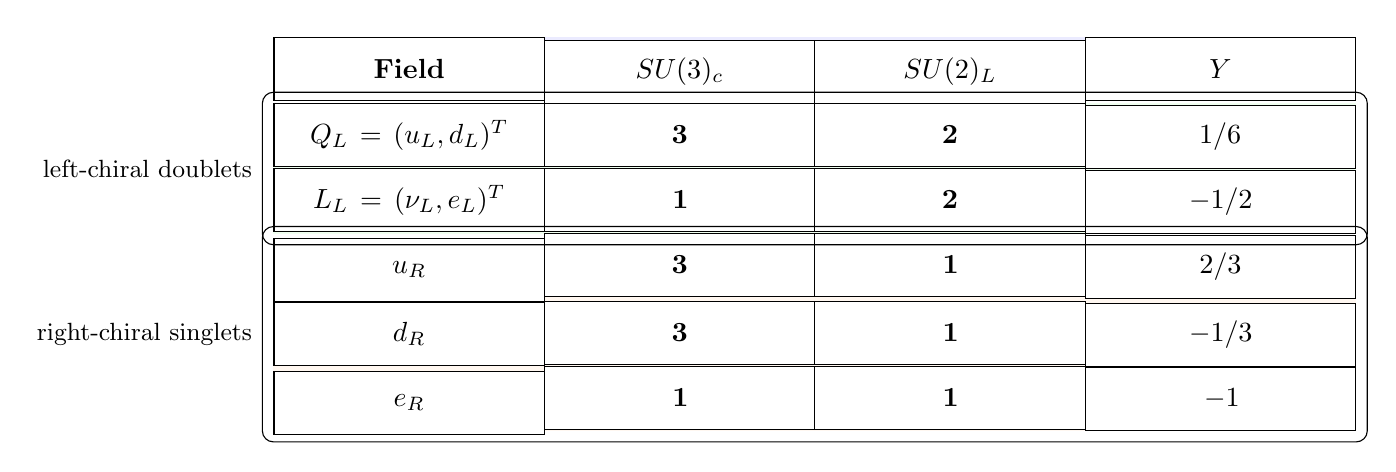
\begin{tikzpicture}
		
		\matrix[
		matrix of nodes,
		nodes={
			draw,
			align=center,
			minimum height=8mm,
			text width=3.2cm,
			fill=white
		},
		row sep=-\pgflinewidth,
		column sep=-\pgflinewidth
		] (m) {
			\textbf{Field} & \textbf{$SU(3)_c$} & \textbf{$SU(2)_L$} & \textbf{$Y$} \\
			$Q_L=(u_L,d_L)^T$ & $\mathbf{3}$ & $\mathbf{2}$ & $1/6$ \\
			$L_L=(\nu_L,e_L)^T$ & $\mathbf{1}$ & $\mathbf{2}$ & $-1/2$ \\
			$u_R$ & $\mathbf{3}$ & $\mathbf{1}$ & $2/3$ \\
			$d_R$ & $\mathbf{3}$ & $\mathbf{1}$ & $-1/3$ \\
			$e_R$ & $\mathbf{1}$ & $\mathbf{1}$ & $-1$ \\
		};
		
		\begin{scope}[on background layer]
			\fill[blue!8]   (m-1-1.north west) rectangle (m-1-4.south east);
			\fill[green!6]  (m-2-1.north west) rectangle (m-3-4.south east);
			\fill[orange!6] (m-4-1.north west) rectangle (m-6-4.south east);
		\end{scope}
		
		\node[
		draw,
		rounded corners,
		fit=(m-2-1)(m-3-4),
		inner sep=4pt,
		label=left:{\small left-chiral doublets}
		] {};
		
		\node[
		draw,
		rounded corners,
		fit=(m-4-1)(m-6-4),
		inner sep=4pt,
		label=left:{\small right-chiral singlets}
		] {};
		
	\end{tikzpicture}
	\caption{One generation of Standard Model fermions organized by representation content.}
	\label{fig:one-generation-expanded}
\end{figure}

\end{comment}




\begin{takehomebox}
\vspace{0.25cm}
A single Standard Model generation already exhibits the essential structure of the theory: color distinguishes quarks from leptons, weak isospin organizes left-chiral doublets, and chirality determines which fields participate in the nontrivial electroweak gauge interaction.
\end{takehomebox}




\section{Hypercharge, weak isospin, and electric charge}

\subsection{The charge operator}

The observed electric charges of quarks and leptons are not assigned independently field by field. In the Standard Model they arise from the relation
\begin{equation}
Q=T_3+Y.
\label{eq:charge-operator-expanded}
\end{equation}
Here \(T_3\) is the third generator of \(\SUw\) and \(Y\) is the weak hypercharge. For a weak doublet, \(T_3\) acts as
\begin{equation}
T_3=\begin{pmatrix}+\half & 0\\ 0 & -\half\end{pmatrix},
\label{eq:T3-doublet-expanded}
\end{equation}
whereas for a weak singlet one has \(T_3=0\).




\subsection{Lepton-sector charge assignments}

For the lepton doublet
\[
L_L=\begin{pmatrix}\nu_L\\ e_L\end{pmatrix},
\qquad Y(L_L)=-\half,
\]
we obtain
\begin{equation}
Q(\nu_L)=+\half-\half=0,
\qquad
Q(e_L)=-\half-\half=-1.
\label{eq:lepton-charges-expanded}
\end{equation}
For the right-chiral charged lepton, which is a weak singlet, \(T_3=0\), so
\begin{equation}
Q(e_R)=0+(-1)=-1.
\label{eq:eR-charge-expanded}
\end{equation}




\subsection{Quark-sector charge assignments}

For the quark doublet
\[
Q_L=\begin{pmatrix}u_L\\ d_L\end{pmatrix},
\qquad Y(Q_L)=\frac16,
\]
we find
\begin{equation}
Q(u_L)=+\half+\frac16=\frac23,
\qquad
Q(d_L)=-\half+\frac16=-\frac13.
\label{eq:quark-doublet-charges-expanded}
\end{equation}
For the right-chiral singlets, \(T_3=0\), so
\begin{equation}
Q(u_R)=\frac23,
\qquad
Q(d_R)=-\frac13.
\label{eq:quark-singlet-charges-expanded}
\end{equation}

\begin{examplebox}{Explicit one-generation charge checks}{example-charge-checks-expanded}
Using \(Q=T_3+Y\), the electric charges of one Standard Model generation are
\[
Q(\nu_L)=0,
\qquad
Q(e_L)=Q(e_R)=-1,
\]
\[
Q(u_L)=Q(u_R)=\frac23,
\qquad
Q(d_L)=Q(d_R)=-\frac13.
\]
Thus the familiar charges of leptons and quarks emerge directly from weak isospin and hypercharge.
\end{examplebox}

\begin{table}[H]
\centering
\caption{Charge checks for one Standard Model generation using \(Q=T_3+Y\).}
\label{tab:charge-checks-clean}
\begin{tabular}{cccc}
\toprule
Field & \(T_3\) & \(Y\) & \(Q=T_3+Y\) \\
\midrule
\(\nu_L\) & \(+\frac12\) & \(-\frac12\) & \(0\) \\
\(e_L\) & \(-\frac12\) & \(-\frac12\) & \(-1\) \\
\(e_R\) & \(0\) & \(-1\) & \(-1\) \\
\(u_L\) & \(+\frac12\) & \(\frac16\) & \(\frac23\) \\
\(d_L\) & \(-\frac12\) & \(\frac16\) & \(-\frac13\) \\
\(u_R\) & \(0\) & \(\frac23\) & \(\frac23\) \\
\(d_R\) & \(0\) & \(-\frac13\) & \(-\frac13\) \\
\bottomrule
\end{tabular}
\end{table}




\subsection{Why these quantum numbers are not arbitrary}

The hypercharges in the Standard Model may look strange at first sight, especially the fractional values carried by the quarks. But one of the main lessons of the theory is that these numbers are not decorative. They are chosen so that the electric charges come out correctly, the chiral structure of the electroweak sector works consistently, and the quantum theory remains anomaly free. The exact anomaly-cancellation story lies beyond the main scope of this module, but the message already belongs here: the quantum numbers are constrained by structure and consistency.




\begin{comment}
	content...
\begin{figure}[H]
\centering
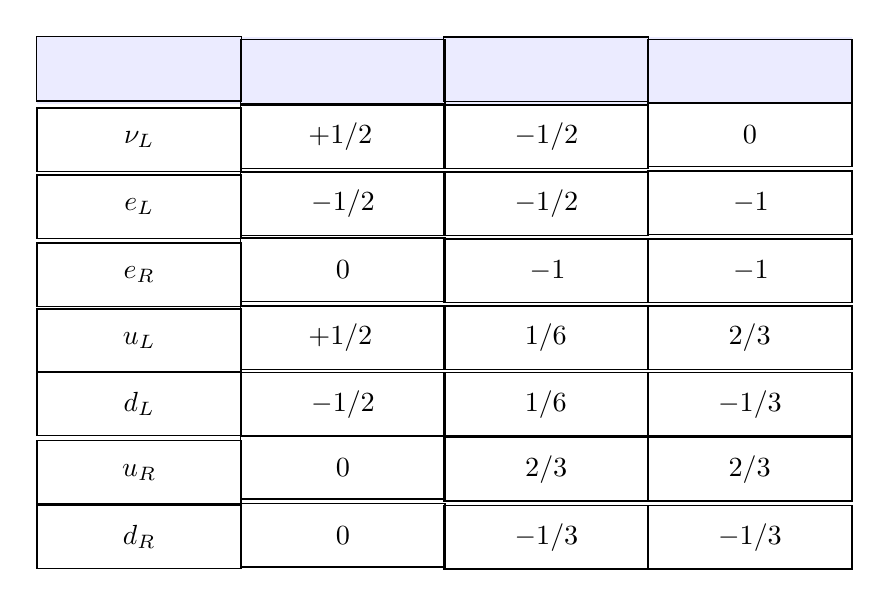
\begin{tikzpicture}
	\matrix[matrix of nodes,nodes={draw,align=center,minimum height=8mm,text width=2.35cm,fill=white},row sep=-\pgflinewidth,column sep=-\pgflinewidth] (m) {
		\textbf{Field} & \textbf{$T_3$} & \textbf{$Y$} & \textbf{$Q=T_3+Y$} \\
		$\nu_L$ & $+1/2$ & $-1/2$ & $0$ \\
		$e_L$ & $-1/2$ & $-1/2$ & $-1$ \\
		$e_R$ & $0$ & $-1$ & $-1$ \\
		$u_L$ & $+1/2$ & $1/6$ & $2/3$ \\
		$d_L$ & $-1/2$ & $1/6$ & $-1/3$ \\
		$u_R$ & $0$ & $2/3$ & $2/3$ \\
		$d_R$ & $0$ & $-1/3$ & $-1/3$ \\
	};
	\fill[blue!8] (m-1-1.north west) rectangle (m-1-4.south east);
	\foreach \r in {1,...,8}{\foreach \c in {1,...,4}{\draw (m-\r-\c.north west) rectangle (m-\r-\c.south east);}}
\end{tikzpicture}
\caption{Electric charge assignments from weak isospin and hypercharge.}
\label{fig:charge-map-expanded}
\end{figure}

\end{comment}


\begin{takehomebox}
\vspace{0.25cm}
The familiar electric charges of quarks and leptons are not independent input data. In the Standard Model they arise from the algebraic relation \(Q=T_3+Y\) once the gauge representations and hypercharges are fixed.
\end{takehomebox}



\begin{guidedchecksbox}
\vspace{0.25cm}
\begin{enumerate}[leftmargin=1.6em,label=\arabic*.]
    \item Reproduce the charge of \(u_L\) and \(d_L\) using \eqref{eq:charge-operator-expanded}.
    \item Check that left- and right-chiral charged leptons have the same electric charge even though they transform differently under \(\SUw\).
    \item Explain why the weak-isospin generator \(T_3\) vanishes on a weak singlet.
\end{enumerate}
\end{guidedchecksbox}




\section{Gauge interactions of Standard Model fields}

\subsection{The Standard Model covariant derivative}

The full Standard Model covariant derivative is obtained by applying the general gauge-theory logic to each factor of the direct-product group
\[
G_{\text{SM}}=\SUc\times\SUw\times U(1)_Y.
\]
Each gauge factor contributes its own connection term:
\begin{itemize}[leftmargin=1.7em]
	\item \(\SUc\) contributes the color gauge field \(G_\mu^a\) with coupling \(g_s\),
	\item \(\SUw\) contributes the weak gauge fields \(W_\mu^i\) with coupling \(g\),
	\item \(U(1)_Y\) contributes the Abelian hypercharge gauge field \(B_\mu\) with coupling \(g'\).
\end{itemize}

In the unbroken phase, the Standard Model covariant derivative takes the form
\begin{equation}
	D_\mu=
	\p_\mu
	-\ii g_s G_\mu^aT^a
	-\ii gW_\mu^i\frac{\tau^i}{2}
	-\ii g' Y B_\mu.
	\label{eq:sm-covariant-derivative-expanded}
\end{equation}
Here \(T^a\) denotes the \(\SUc\) generators acting on color indices, while \(\tau^i/2\) are the \(\SUw\) generators in the weak-doublet representation. For the Abelian factor \(U(1)_Y\), the generator acts simply by multiplication by the hypercharge number \(Y\) carried by the field.

Therefore the full covariant derivative is the ordinary derivative plus one gauge contribution for each local symmetry factor. In that sense, the Standard Model covariant derivative is not guessed independently: it is the direct-product version of the Abelian and Yang--Mills constructions developed earlier.
This one formula contains the entire gauge interaction structure of the Standard Model at the kinetic level. But its interpretation depends on the field to which it is applied.



\subsection{Field-by-field application: quark sector}

Before writing the explicit covariant derivative, it is worth reading the representation label carefully. The assignment
\[
Q_L:(\mathbf{3},\mathbf{2})_{1/6}
\]
means that \(Q_L\) is:
\begin{itemize}[leftmargin=1.7em]
\item a triplet of \(\SUc\), so the color generators \(T^a\) act nontrivially;
\item a doublet of \(\SUw\), so the weak generators are \(T_L^i=\tau^i/2\);
\item a field of hypercharge \(Y=1/6\), so the Abelian \(U(1)_Y\) term is proportional to \(1/6\).
\end{itemize}
This is why all three gauge terms appear in \(D_\mu Q_L\).

For the left-chiral quark doublet \(Q_L:(\mathbf{3},\mathbf{2})_{1/6}\), all three gauge sectors act nontrivially. Its covariant derivative is
\begin{equation}
D_\mu Q_L=
\left(
\p_\mu-\ii g_s G_\mu^aT^a-\ii gW_\mu^i\frac{\tau^i}{2}-\ii g'\frac16 B_\mu
\right)Q_L.
\label{eq:Dmu-QL-expanded}
\end{equation}
The right-chiral quark singlets are weak singlets but still carry color and hypercharge:
\begin{align}
D_\mu u_R &=
\left(\p_\mu-\ii g_s G_\mu^aT^a-\ii g'\frac23 B_\mu\right)u_R,
\label{eq:Dmu-uR-expanded}\\
D_\mu d_R &=
\left(\p_\mu-\ii g_s G_\mu^aT^a+\ii g'\frac13 B_\mu\right)d_R.
\label{eq:Dmu-dR-expanded}
\end{align}

The logic for the right-chiral quark singlets is parallel, but simpler. The assignments
\[
u_R:(\mathbf{3},\mathbf{1})_{2/3},
\qquad
d_R:(\mathbf{3},\mathbf{1})_{-1/3}
\]
say that these fields are still color triplets and therefore still couple to the gluons, but they are weak singlets and therefore carry no nontrivial \(\SUw\) generators. That is why the \(W_\mu^i\tau^i/2\) term is absent from \eqref{eq:Dmu-uR-expanded} and \eqref{eq:Dmu-dR-expanded}, while the \(\SUc\) and \(U(1)_Y\) terms remain.
The quark sector therefore couples to color, weak isospin, and hypercharge, but the \(\SUw\) coupling is present only for the left-chiral doublet.

It is also useful to see explicitly how the gauge interactions arise from the kinetic term. For the left-chiral quark doublet,
\begin{align}
	\bar Q_L \ii \gmu D_\mu Q_L
	&=
	\bar Q_L \ii \gmu \p_\mu Q_L
	+ g_s \bar Q_L \gmu G_\mu^a T^a Q_L
	+ g \bar Q_L \gmu W_\mu^i \frac{\tau^i}{2} Q_L
	+ g' \frac16 \bar Q_L \gmu B_\mu Q_L.
	\label{eq:QL-kinetic-expanded-to-interactions}
\end{align}
The first term is the free kinetic term, while the remaining terms are the gauge interactions with gluons, weak gauge bosons, and the hypercharge gauge field. Thus the interaction terms are not added by hand: they are generated automatically once \(\p_\mu\) is replaced by \(D_\mu\).


\subsection{Field-by-field application: lepton sector}

The lepton assignments should be read in exactly the same way. The label
\[
L_L:(\mathbf{1},\mathbf{2})_{-1/2}
\]
means that \(L_L\) is a color singlet, a weak doublet, and has hypercharge \(-1/2\). Because it is a singlet of \(\SUc\), the color generators vanish on it. By contrast, the label
\[
e_R:(\mathbf{1},\mathbf{1})_{-1}
\]
means that \(e_R\) is both a color singlet and a weak singlet, but still carries nonzero hypercharge.

For the left-chiral lepton doublet \(L_L:(\mathbf{1},\mathbf{2})_{-1/2}\), the color generators vanish, so one finds
\begin{equation}
D_\mu L_L=
\left(
\p_\mu-\ii gW_\mu^i\frac{\tau^i}{2}+\ii g'\frac12 B_\mu
\right)L_L.
\label{eq:Dmu-LL-expanded}
\end{equation}
For the right-chiral charged lepton,
\begin{equation}
D_\mu e_R=(\p_\mu+\ii g'B_\mu)e_R.
\label{eq:Dmu-eR-expanded}
\end{equation}
The right-chiral charged lepton is particularly instructive. Since \(e_R\) is a weak singlet, the \(\SUw\) generators act trivially on it, so there is no term involving \(W_\mu^i\tau^i/2\) in \eqref{eq:Dmu-eR-expanded}. Since it is also color neutral, there is no gluon term either. What remains is only the ordinary derivative and the Abelian hypercharge contribution.  
Again the pattern is clear: the left-chiral lepton doublet feels the weak-isospin interaction, but the right-chiral charged lepton does not. Both, however, couple to hypercharge in the unbroken theory.



\subsection{Higgs as a gauge multiplet before symmetry breaking}

Even before one discusses spontaneous symmetry breaking, the Higgs field is already part of the gauge-theory field content. In the Standard Model it transforms as
\begin{equation}
H=\begin{pmatrix}H^+\\ H^0\end{pmatrix},
\qquad
H:(\mathbf{1},\mathbf{2})_{1/2}.
\label{eq:Higgs-representation-expanded}
\end{equation}

The assignment
\[
H:(\mathbf{1},\mathbf{2})_{1/2}
\]
means that the Higgs field is color neutral, transforms as a weak doublet, and carries hypercharge \(1/2\). Using the convention \(Q=T_3+Y\), one can already check the electric charges of its two components:
\begin{equation}
	Q(H^+) = +\frac12 + \frac12 = +1,
	\qquad
	Q(H^0) = -\frac12 + \frac12 = 0.
	\label{eq:Higgs-charge-check}
\end{equation}
This assignment is also the one needed for the Higgs field to participate in gauge-invariant Yukawa couplings to charged fermions in the full Standard Model. The detailed Yukawa construction belongs later, but it is useful already now to note that the Higgs quantum numbers are not decorative: they are tightly linked to the electroweak structure of the theory. 
So the notation \(H^+\) and \(H^0\) is already fixed by weak isospin and hypercharge, even before electroweak symmetry breaking is discussed.

Its covariant derivative is therefore
\begin{equation}
D_\mu H=
\left(
\p_\mu-\ii gW_\mu^i\frac{\tau^i}{2}-\ii g'\frac12 B_\mu
\right)H.
\label{eq:Dmu-Higgs-expanded}
\end{equation}
At the present stage this simply tells us that the Higgs field is an electroweak doublet carrying hypercharge. The dynamical consequences of its vacuum expectation value belong later.

\begin{examplebox}{Applying \texorpdfstring{$D_\mu$}{Dmu} explicitly to representative multiplets}{example-Dmu-representatives}
For the left-chiral quark doublet,
\[
D_\mu Q_L=
\left(
\p_\mu-\ii g_s G_\mu^aT^a-\ii gW_\mu^i\frac{\tau^i}{2}-\ii g'\frac16 B_\mu
\right)Q_L.
\]
For the left-chiral lepton doublet,
\[
D_\mu L_L=
\left(
\p_\mu-\ii gW_\mu^i\frac{\tau^i}{2}+\ii g'\frac12 B_\mu
\right)L_L.
\]
For the right-chiral charged lepton,
\[
D_\mu e_R=(\p_\mu+\ii g'B_\mu)e_R.
\]
These formulas make visible, field by field, which gauge sectors are active.
\end{examplebox}



\subsection{Physical interpretation of the gauge couplings}


At this point it is important to avoid a common first misunderstanding. The fact that the Standard Model has one general structural formula for \(D_\mu\) does \emph{not} mean that all gauge bosons couple to all fields. Which terms survive in the covariant derivative depends entirely on the representation carried by the field. The gauge group is universal; the active couplings are representation dependent. 
Equation \eqref{eq:sm-covariant-derivative-expanded} answers a basic physical question in a very economical way: which Standard Model fields couple to which gauge bosons? The answer is immediate from the representations.
\begin{itemize}[leftmargin=1.7em]
\item Only quarks couple to the gluons, because only quarks carry color.
\item Only left-chiral doublets couple nontrivially to the weak \(\SUw\) gauge fields.
\item All fields with nonzero hypercharge couple to \(B_\mu\).
\end{itemize}

A useful comparison is:
\begin{itemize}[leftmargin=1.7em]
\item \(Q_L:(\mathbf{3},\mathbf{2})_{1/6}\) couples to gluons, weak gauge bosons, and \(B_\mu\);
\item \(L_L:(\mathbf{1},\mathbf{2})_{-1/2}\) couples to weak gauge bosons and \(B_\mu\), but not to gluons;
\item \(e_R:(\mathbf{1},\mathbf{1})_{-1}\) couples only to \(B_\mu\).
\end{itemize}
This side-by-side comparison makes visible how the representation labels directly determine which pieces of the full Standard Model gauge structure act on a given field.

Thus the gauge interaction pattern is not tabulated by hand. It is encoded in the covariant derivative once the field content is known.

\begin{remarkbox}{The same \texorpdfstring{$D_\mu$}{Dmu} does not act identically on every field}{remark-Dmu-not-identical}
The covariant derivative has one general structural form, but the actual matrices appearing in it depend on the representation of the field. For a color singlet, the \(\SUc\) generators vanish. For a weak singlet, the \(\SUw\) generators vanish. For a field with hypercharge \(Y\), the Abelian term is simply proportional to that number. Representation theory therefore determines the gauge couplings field by field.
\end{remarkbox}



\begin{takehomebox}
\vspace{0.25cm}
The Standard Model covariant derivative packages the entire gauge interaction structure of the theory. Once the gauge group and the representations of the matter fields are known, the couplings to gluons, weak gauge bosons, and hypercharge follow directly.
\end{takehomebox}

\begin{guidedchecksbox}
\vspace{0.25cm}
\begin{enumerate}[leftmargin=1.6em,label=\arabic*.]
    \item Explain why there is no color term in \eqref{eq:Dmu-LL-expanded}.
    \item Explain why there is no weak-isospin term in \eqref{eq:Dmu-uR-expanded}, \eqref{eq:Dmu-dR-expanded}, and \eqref{eq:Dmu-eR-expanded}.
    \item Identify which gauge fields couple to the Higgs doublet in the unbroken phase.
\end{enumerate}
\end{guidedchecksbox}





\section{The gauge-sector Lagrangian of the Standard Model before symmetry breaking}

\subsection{Gauge kinetic terms}



Each factor of the Standard Model gauge group contributes its own gauge-field kinetic term. For the Abelian hypercharge sector,
\begin{equation}
\Lag_Y=-\frac14 B_{\mu\nu}B^{\mu\nu},
\qquad
B_{\mu\nu}=\p_\mu B_\nu-\p_\nu B_\mu.
\label{eq:hypercharge-kinetic-expanded}
\end{equation}

The gauge kinetic sector is not guessed independently. It is inherited factor by factor from the general gauge-theory structures derived earlier in the note. The Abelian \(U(1)_Y\) factor contributes the Maxwell-like field strength \(B_{\mu\nu}\), while the non-Abelian \(\SUw\) and \(\SUc\) factors contribute Yang--Mills field strengths containing quadratic gauge-field terms. The Standard Model gauge kinetic sector is therefore the direct-product sum of one Abelian and two non-Abelian pieces.

For the weak sector,
\begin{equation}
\Lag_W=-\frac14 W_{\mu\nu}^iW^{i\mu\nu},
\qquad
W_{\mu\nu}^i=\p_\mu W_\nu^i-\p_\nu W_\mu^i+g\epsilon^{ijk}W_\mu^jW_\nu^k.
\label{eq:weak-kinetic-expanded}
\end{equation}
For the color sector,
\begin{equation}
\Lag_G=-\frac14 G_{\mu\nu}^aG^{a\mu\nu},
\qquad
G_{\mu\nu}^a=\p_\mu G_\nu^a-\p_\nu G_\mu^a+g_sf^{abc}G_\mu^bG_\nu^c.
\label{eq:color-kinetic-expanded}
\end{equation} 
The structural difference between the Abelian and non-Abelian sectors is now visible in the field strengths themselves. The Abelian tensor \(B_{\mu\nu}\) is linear in the gauge field because \(U(1)_Y\) has commuting generators. By contrast, \(W_{\mu\nu}^i\) and \(G_{\mu\nu}^a\) contain terms quadratic in the gauge fields because \(\SUw\) and \(\SUc\) are Yang--Mills theories. When substituted into \(\Lag_W\) and \(\Lag_G\), these quadratic pieces generate cubic and quartic gauge-boson self-interactions. 
These terms show already that the non-Abelian sectors contain self-interactions of the gauge fields, while the Abelian hypercharge sector does not.




\subsection{Fermion kinetic terms with covariant derivatives}

For one generation, the fermion kinetic sector is
\begin{align}
\Lag_{\text{fermion}}
&=
\bar Q_L\ii\gmu D_\mu Q_L + \bar u_R\ii\gmu D_\mu u_R + \bar d_R\ii\gmu D_\mu d_R
\nonumber\\
&\qquad
+\bar L_L\ii\gmu D_\mu L_L + \bar e_R\ii\gmu D_\mu e_R.
\label{eq:fermion-kinetics-expanded}
\end{align}
Conceptually, the fermion kinetic sector is obtained by taking the free relativistic kinetic term for each matter field and replacing the ordinary derivative by the gauge-covariant derivative. This is the Standard Model realization of the same gauge-principle step already seen in QED and Yang--Mills theory: once local gauge invariance is imposed, the kinetic terms automatically generate the admissible gauge interactions. 
For example, the quark-doublet kinetic term expands as
\begin{align}
	\bar Q_L \ii \gmu D_\mu Q_L
	&=
	\bar Q_L \ii \gmu \p_\mu Q_L
	+ g_s \bar Q_L \gmu G_\mu^a T^a Q_L
	+ g \bar Q_L \gmu W_\mu^i \frac{\tau^i}{2} Q_L
	+ g' \frac16 \bar Q_L \gmu B_\mu Q_L.
	\label{eq:fermion-kinetic-example-QL}
\end{align}
This makes explicit how the kinetic term contains both the free propagation piece and the gauge interaction terms.

For the full Standard Model, one sums this structure over the three generations. The crucial point for Module~3 is not flavor yet, but the gauge-covariant form of the kinetic terms.



\subsection{The Higgs field as part of the pre-EWSB gauge theory}

The Higgs field enters the gauge theory before symmetry breaking simply as another matter multiplet with electroweak quantum numbers. Its kinetic term is
\begin{equation}
\Lag_H=(D_\mu H)^\dagger(D^\mu H).
\label{eq:Higgs-kinetic-expanded}
\end{equation}
At a schematic level, substituting the electroweak covariant derivative into \(\Lag_H\) gives
\begin{align}
	(D_\mu H)^\dagger(D^\mu H)
	&=
	(\p_\mu H)^\dagger(\p^\mu H)
	+ \text{terms linear in } W_\mu^i \text{ and } B_\mu
	+ \text{terms quadratic in } W_\mu^i \text{ and } B_\mu .
	\label{eq:Higgs-kinetic-schematic-expansion}
\end{align}
So even in the unbroken theory, the Higgs field is not an isolated scalar added later for mass generation. It is already an electroweak matter multiplet that transforms under \(\SUw\times U(1)_Y\) and therefore already participates in the gauge dynamics. 
The first term is the free Higgs kinetic term, while the additional terms show that the Higgs field already interacts with the electroweak gauge bosons before symmetry breaking is discussed. 
Thus, even before one studies the Higgs mechanism, the Higgs field already belongs naturally to the gauge-theory field content and participates in the electroweak covariant derivative.



\subsection{What is already fixed before electroweak symmetry breaking}

Collecting the gauge kinetic terms, fermion kinetic terms, and Higgs kinetic term, one may write the gauge-invariant Standard Model Lagrangian before symmetry breaking schematically as
\begin{equation}
\Lag_{\text{SM}}^{\text{(gauge phase)}}=
-\frac14 G_{\mu\nu}^aG^{a\mu\nu}
-\frac14 W_{\mu\nu}^iW^{i\mu\nu}
-\frac14 B_{\mu\nu}B^{\mu\nu}
+\Lag_{\text{fermion}}
+(D_\mu H)^\dagger(D^\mu H)
+\cdots.
\label{eq:sm-gauge-phase-expanded}
\end{equation}
The phrase \textit{before electroweak symmetry breaking} should be interpreted carefully. At this stage, the local gauge group, the field content, the representation assignments, and the gauge-covariant kinetic terms are already fixed. What has \emph{not} yet been specified is the symmetry-breaking vacuum and the resulting reorganization into physical massive and massless gauge-boson combinations. In other words, the gauge architecture is already in place; the later Higgs mechanism changes the vacuum structure and the physical interpretation of part of that gauge sector. 
The ellipsis denotes terms such as the Higgs potential and the Yukawa couplings, whose full role becomes clear only when spontaneous symmetry breaking is studied.

Nevertheless, a large part of the Standard Model is already fixed at this stage:
\begin{itemize}[leftmargin=1.7em]
    \item the gauge group,
    \item the gauge fields,
    \item the field strengths,
    \item the matter multiplets,
    \item the covariant derivatives,
    \item and the kinetic gauge interactions.
\end{itemize}
This is why it is correct to say that the Standard Model is already highly constrained before one even begins to discuss masses and mixing.



\begin{remarkbox}{What is fixed before symmetry breaking}{remark-fixed-before-ewsb-expanded}
Even before the Higgs mechanism is invoked, the Standard Model already possesses a rigid gauge-theoretic architecture. The local symmetry group, the field content, the representation assignments, and the gauge-covariant kinetic terms are fixed. Electroweak symmetry breaking later changes the vacuum and the interpretation of the neutral gauge fields, but it does not create the gauge structure from scratch.
\end{remarkbox}



\begin{takehomebox}
\vspace{0.25cm}
The Standard Model before electroweak symmetry breaking is already a tightly constrained chiral gauge theory. The later Higgs mechanism acts on an interaction structure that is already in place.
\end{takehomebox}



\begin{guidedchecksbox}
\vspace{0.25cm}
\begin{enumerate}[leftmargin=1.6em,label=\arabic*.]
    \item Identify which terms in \eqref{eq:sm-gauge-phase-expanded} come from Abelian gauge theory and which from non-Abelian Yang--Mills theory.
    \item Explain why the Higgs kinetic term belongs naturally in a gauge-theory discussion even before symmetry breaking is studied.
    \item List three structural ingredients of the Standard Model that are already fixed before the Higgs mechanism enters.
\end{enumerate}
\end{guidedchecksbox}





\section{Why the Standard Model is constrained rather than arbitrary}



\subsection{Interactions follow from symmetry rather than from guesswork}



The Standard Model is not built by first listing particles and then writing down plausible interaction terms one by one. Instead, once the gauge group {\color{red}\(\SMgauge\)} is specified and the matter fields are assigned to definite representations, a large part of the interaction structure is already determined. The logic can be summarized compactly:
\begin{itemize}[leftmargin=1.7em]
    \item a global internal symmetry gives a conserved current,
    \item promoting it to a local symmetry makes the ordinary derivative fail,
    \item restoring covariance forces the introduction of gauge fields,
    \item the representation of each matter field determines which gauge fields act on it,
    \item the gauge-covariant kinetic terms then generate the admissible gauge interactions.
\end{itemize}
Thus the interaction structure is not guessed; it is constructed.




\subsection{Representations determine couplings}

One of the most economical features of the Standard Model is that the pattern of interactions is encoded in the representation content. Quarks couple to gluons because they carry color; leptons do not because they are color singlets. Left-chiral weak doublets couple nontrivially to \(\SUw\), whereas right-chiral weak singlets do not. Fields with nonzero hypercharge couple to \(B_\mu\), while fields with vanishing hypercharge would not.

What initially looks like a complicated table of fields and couplings is therefore the visible expression of a smaller number of structural inputs: gauge group, representation assignments, and local invariance.



\subsection{Non-Abelian symmetry adds further rigidity}

The Standard Model is even more constrained than QED because two of its gauge factors are non-Abelian. The commutator term in the Yang--Mills field strength forces gauge-boson self-interactions and thereby makes the gauge sector itself richer than in the Abelian case. This is already true at the formal level, before any phenomenology is discussed.



\subsection{Chirality sharpens the electroweak structure}

The electroweak sector is a chiral gauge theory. This left-right asymmetry is not a small technical detail but one of the most rigid features of the Standard Model. It explains why weak interactions violate parity and why naive fermion mass terms are not gauge invariant before symmetry breaking.


\begin{remarkbox}{A preview of the mass problem}{remark-mass-problem-expanded}
A fermion mass term couples left- and right-chiral components. In the Standard Model these components do not transform identically under \(\SUw\times\UY\). As a result, a naive mass term would spoil gauge invariance in the unbroken phase. This is one of the deep reasons why the Higgs field is needed, and it is the natural bridge to Module~5.
\end{remarkbox}



\subsection{A brief advanced remark on consistency and anomalies}

There is a further sense in which the Standard Model is constrained. In a chiral gauge theory, quantum effects may generate anomalies. If gauge anomalies failed to cancel, the quantum theory would be inconsistent. The hypercharges and representation assignments of the Standard Model are therefore not arbitrary decorations. They form a delicate pattern that allows the potentially dangerous quantum contributions to cancel.

A full derivation of anomaly cancellation lies beyond the main scope of Module~3, but the conceptual lesson belongs here: the Standard Model is constrained not only by classical local symmetry but also by quantum consistency.



\begin{remarkbox}{Anomaly cancellation as a structural clue}{remark-anomaly-clue-expanded}
The fractional hypercharges of the Standard Model may look puzzling at first sight, but they are part of a tightly coordinated pattern. Their role is not only to reproduce the observed electric charges through \(Q=T_3+Y\), but also to keep the quantum theory consistent.
\end{remarkbox}



\begin{takehomebox}
\vspace{0.25cm}
The Standard Model is constrained at several levels simultaneously: local symmetry fixes the form of gauge interactions, representations determine which fields couple to which sectors, non-Abelian structure forces gauge-boson self-interactions, and quantum consistency places further restrictions on the matter content and hypercharges.
\end{takehomebox}




\section{Bridge to the later modules}

\subsection{From gauge structure to strong-interaction physics: Module~4}


In the present module, \(\SUc\) has appeared as one factor in the Standard Model gauge group and the gluon fields have been introduced through the non-Abelian covariant derivative and field strength. But this is only the structural beginning of the strong interaction. Module~4 develops what the \(\SUc\) Yang--Mills theory actually does physically: asymptotic freedom, running coupling, confinement, hadrons, and jet physics.



\subsection{From gauge symmetry to mass generation: Module~5}

The electroweak sector has also been constructed here only in its unbroken gauge form. We have introduced \(\SUw\times\UY\), the gauge fields \(W_\mu^i\) and \(B_\mu\), the fermion multiplets, and the Higgs doublet as a gauge multiplet. But we have not yet answered how the \(W\) and \(Z\) bosons acquire mass while preserving the gauge structure of the theory. That question belongs to Module~5 and is addressed through spontaneous symmetry breaking and the Higgs mechanism.



\subsection{From the Lagrangian to observables: Module~6}

A theory becomes physics when it is connected to measurable quantities. Module~3 is intentionally structural: it emphasizes the logic of the gauge construction. Module~6 will translate that structure into Feynman rules, amplitudes, decay widths, and cross sections. Thus the formal work done here is not an abstract detour; it is the foundation of the later phenomenological machinery.




\begin{figure}[H]
\centering
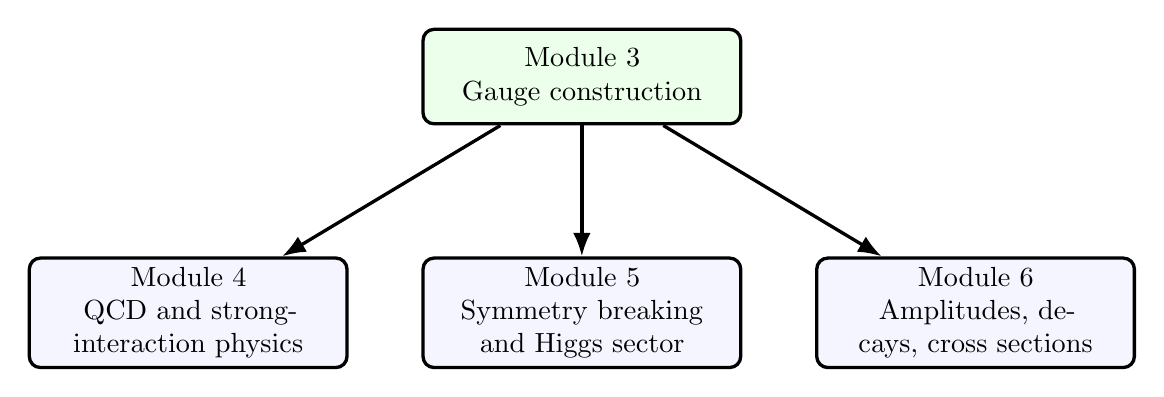
\begin{tikzpicture}[
	block/.style={rounded corners, draw=black, very thick, align=center, minimum height=1.2cm, text width=3.8cm, fill=blue!4},
	arr/.style={-{Latex[length=3mm]}, very thick}
	]
	\node[block, fill=green!8] (m3) at (0,0) {Module 3\\Gauge construction};
	\node[block] (m4) at (-5.0,-3.0) {Module 4\\QCD and strong-interaction physics};
	\node[block] (m5) at (0,-3.0) {Module 5\\Symmetry breaking and Higgs sector};
	\node[block] (m6) at (5.0,-3.0) {Module 6\\Amplitudes, decays, cross sections};
	\draw[arr] (m3) -- (m4);
	\draw[arr] (m3) -- (m5);
	\draw[arr] (m3) -- (m6);
\end{tikzpicture}
\caption{Conceptual bridge from Module~3 to the later modules of the course.}
\label{fig:bridge-later-modules-expanded}
\end{figure}




\begin{takehomebox}
\vspace{0.25cm}
Module~3 constructs the gauge-theoretic framework of the Standard Model. Module~4 turns \(\SUc\) into QCD physics. Module~5 explains how electroweak symmetry breaking produces the observed mass pattern. Module~6 translates the Lagrangian into measurable amplitudes and observables.
\end{takehomebox}



\section{Final summary and conceptual map}

\subsection{The logical chain of the module}

The central thread running through the module can now be restated in its full form:
\[
\begin{aligned}
\text{global symmetry}
&\longrightarrow \text{local symmetry}
\longrightarrow \text{failure of }\p_\mu
\longrightarrow \text{covariant derivative} \\
&\longrightarrow \text{gauge field}
\longrightarrow \text{field strength}
\longrightarrow \text{gauge-invariant Lagrangian}.
\end{aligned}
\]
and then, by generalization,
\[
\begin{aligned}
\text{QED}
&\longrightarrow \text{Yang--Mills theory}
\longrightarrow \text{Standard Model gauge structure} \\
&\longrightarrow \text{matter multiplets}
\longrightarrow \text{charge assignments}
\longrightarrow \text{pre-EWSB gauge Lagrangian}.
\end{aligned}
\]
If this chain is understood as one connected argument, then the main conceptual goal of the module has been achieved.




\subsection{The Standard Model is not a particle catalogue}

A particle chart is useful, but it hides the deepest pedagogical lesson of the Standard Model. The theory is best understood not as ``particles plus forces'' but as a relativistic chiral gauge theory with a specific local symmetry group, specific matter representations, and a tightly constrained interaction structure. The particle content is the visible surface of a deeper gauge-theoretic organization.



\subsection{What the student should now be able to see}

After completing this module, a student should be able to see the following statements as parts of one coherent picture rather than disconnected facts:
\begin{itemize}[leftmargin=1.7em]
    \item local symmetry requires gauge fields,
    \item QED is the simplest complete gauge theory,
    \item non-Abelian symmetry forces gauge-boson self-interactions,
    \item the Standard Model gauge group determines the broad pattern of interactions,
    \item the matter multiplets encode the coupling structure,
    \item electric charge emerges from \(Q=T_3+Y\),
    \item chirality is central to the electroweak sector.
\end{itemize}

\begin{takehomebox}
\vspace{0.25cm}
The Standard Model is not best understood as a list of particles and forces. It is best understood as a relativistic chiral gauge theory whose local symmetry group, field content, and representation structure tightly constrain the form of the interactions. Module~3 is the stage of the course where that logic becomes visible.
\end{takehomebox}

\appendix




\section{Conventions summary}

For quick reference, the main conventions used in these notes are:
\begin{itemize}[leftmargin=1.7em]
\item \(\eta_{\mu\nu}=\diag(1,-1,-1,-1)\),
\item \(\acomm{\gamma^\mu}{\gamma^\nu}=2\eta^{\mu\nu}\),
\item \(\PL=(1-\gamma^5)/2\), \(\PR=(1+\gamma^5)/2\),
\item Abelian case: \(D_\mu=\p_\mu-\ii q A_\mu\),
\item Non-Abelian case: \(D_\mu=\p_\mu-\ii g A_\mu\), with \(A_\mu=A_\mu^aT^a\),
\item Hypercharge convention: \(Q=T_3+Y\),
\item Standard Model gauge group: {\color{red}\(G_{\text{SM}}=\SMgauge\)}.
\end{itemize}





\section{One-generation field table}


\begin{center}
\begin{tabular}{>{\raggedright\arraybackslash}p{0.24\textwidth}ccc}
\toprule
Field & \(\SUc\) & \(\SUw\) & \(Y\) \\
\midrule
\(Q_L\) & \(\mathbf{3}\) & \(\mathbf{2}\) & \(\frac16\) \\
\(L_L\) & \(\mathbf{1}\) & \(\mathbf{2}\) & \(-\frac12\) \\
\(u_R\) & \(\mathbf{3}\) & \(\mathbf{1}\) & \(\frac23\) \\
\(d_R\) & \(\mathbf{3}\) & \(\mathbf{1}\) & \(-\frac13\) \\
\(e_R\) & \(\mathbf{1}\) & \(\mathbf{1}\) & \(-1\) \\
\(H\) & \(\mathbf{1}\) & \(\mathbf{2}\) & \(\frac12\) \\
\bottomrule
\end{tabular}
\end{center}



\section{Guided-check summary}

For convenience, the main guided checks of the note are collected conceptually here:
\begin{itemize}[leftmargin=1.7em]
    \item verify the invariance of the free Dirac Lagrangian under global \(U(1)\),
    \item derive the Noether current and continuity equation,
    \item check the transformation of \(\p_\mu\psi\) under local \(U(1)\),
    \item verify the Abelian field-strength transformation,
    \item derive the non-Abelian field strength from the commutator \([D_\mu,D_\nu]\),
    \item reproduce the one-generation charge assignments from \(Q=T_3+Y\),
    \item identify which gauge sectors couple to each Standard Model multiplet.
\end{itemize}

\end{document}


